%%%%%%%%%%%%%%%%%%%%%%%%%%%%%%%%%%%%%%%%%%%%%%%%%%%
%% LaTeX book template                           %%
%% Author:  Amber Jain (http://amberj.devio.us/) %%
%% License: ISC license                          %%
%%%%%%%%%%%%%%%%%%%%%%%%%%%%%%%%%%%%%%%%%%%%%%%%%%%

\documentclass[11pt, fleqn]{book}
\usepackage[b5paper, top=2.5cm, bottom=2.5cm, left=2cm, right=2cm]{geometry} %para personalizar el tamaño y margenes de la hoja
\usepackage[T1]{fontenc}
\usepackage[utf8]{inputenc}
\usepackage{lmodern}
%%%%%%%%%%%%%%%%%%%%%%%%%%%%%%%%%%%%%%%%%%%%%%%%%%%%%%%%%
% Source: http://en.wikibooks.org/wiki/LaTeX/Hyperlinks %
%%%%%%%%%%%%%%%%%%%%%%%%%%%%%%%%%%%%%%%%%%%%%%%%%%%%%%%%%
\usepackage[colorlinks=false]{hyperref}
\usepackage{graphicx}
\usepackage[spanish, es-noshorthands]{babel}

\usepackage{float} %lo agregue para las tablas qeu andaban de rebeldes
\usepackage{amsmath} %lo agregue para la numeración de las Ecuaciones
\usepackage{amsthm}
\usepackage{amsfonts}
\usepackage{mathtools}
\usepackage{amssymb}
\usepackage{stackengine}
\usepackage{graphicx} %para las imagenes
\usepackage{float}
%*************Aun falta el graphics path%
\usepackage{lscape} %necesario para usar la propiedad "begin{landscape}"
\usepackage{longtable} %necesario para usa la propiedad "longtable"
\usepackage{booktabs} %necesario para usar la propiedad "toprule"
\usepackage{mathrsfs}

%%%%%%%%%%%%%%%%%%%%%%%%%%%%%%%%%%%%%%%%%%%%%%%%%%%%%%%%%%%%%%%%%%%%%%%%%%%%%%%%
% 'dedication' environment: To add a dedication paragraph at the start of book %
% Source: http://www.tug.org/pipermail/texhax/2010-June/015184.html            %
%%%%%%%%%%%%%%%%%%%%%%%%%%%%%%%%%%%%%%%%%%%%%%%%%%%%%%%%%%%%%%%%%%%%%%%%%%%%%%%%
% You might want to add short description about each chapter in this book.
%The website\footnote{\url{https://github.com/amberj/latex-book-template}} for this file contains:

\newenvironment{dedication}
{
   \cleardoublepage
   \thispagestyle{empty}
   \vspace*{\stretch{1}}
   \hfill\begin{minipage}[t]{0.66\textwidth}
   \raggedright
}
{
   \end{minipage}
   \vspace*{\stretch{3}}
   \clearpage
}

%%%%%%%%%%%%%%%%%%%%%%%%%%%%%%%%%%%%%%%%%%%%%%%%
% Chapter quote at the start of chapter        %
% Source: http://tex.stackexchange.com/a/53380 %
%%%%%%%%%%%%%%%%%%%%%%%%%%%%%%%%%%%%%%%%%%%%%%%%
%%%%%%%%%%%%%%%%%%%%%%%%%%%%%%%%%%%%
% Give credit where credit is due. %
% Say thanks!                      %
%%%%%%%%%%%%%%%%%%%%%%%%%%%%%%%%%%%%

\makeatletter
\renewcommand{\@chapapp}{}% Not necessary...
\newenvironment{chapquote}[2][2em]
  {\setlength{\@tempdima}{#1}%
   \def\chapquote@author{#2}%
   \parshape 1 \@tempdima \dimexpr\textwidth-2\@tempdima\relax%
   \itshape}
  {\par\normalfont\hfill--\ \chapquote@author\hspace*{\@tempdima}\par\bigskip}
\makeatother

%%%%%%%%%%%%%%%%%%%%%%%%%%%%%%%%%%%%%%%%%%%%%%%%%%%
% First page of book which contains 'stuff' like: %
%  - Book title, subtitle                         %
%  - Book author name                             %
%%%%%%%%%%%%%%%%%%%%%%%%%%%%%%%%%%%%%%%%%%%%%%%%%%%

% Book's title and subtitle
\title{\Huge {Transferencia de masa} }
% Author
\author{\textsc{Octavio Manero Brito}}

\begin{document}

\frontmatter
\maketitle

%%%%%%%%%%%%%%%%%%%%%%%%%%%%%%%%%%%%%%%%%%%%%%%%%%%%%%%%%%%%%%%
% Add a dedication paragraph to dedicate your book to someone %
%%%%%%%%%%%%%%%%%%%%%%%%%%%%%%%%%%%%%%%%%%%%%%%%%%%%%%%%%%%%%%%
\begin{dedication}
Dedicated to Calvin and Hobbes.
\end{dedication}

%%%%%%%%%%%%%%%%%%%%%%%%%%%%%%%%%%%%%%%%%%%%%%%%%%%%%%%%%%%%%%%%%%%%%%%%
% Auto-generated table of contents, list of figures and list of tables %
%%%%%%%%%%%%%%%%%%%%%%%%%%%%%%%%%%%%%%%%%%%%%%%%%%%%%%%%%%%%%%%%%%%%%%%%

\tableofcontents
%\listoffigures
%\listoftables

\mainmatter
%%%%%%%%%%%
% Preface %
%%%%%%%%%%%
\chapter*{Prefacio}


%%%%%%%%%%%%%%%%
% NEW CHAPTER! %
%%%%%%%%%%%%%%%%
\chapter{Capitulo 1}
\section{Lo de los chavalos XD}
AQUÍ va todo lo anterior 
%\section*{esto es una sección}
%\subsection{esto es una subsección}
%\subsubsection{esto es una subsubsección}
%\begin{itemize}
%\item mi primer item 
%\item mi seguendo item
%\end{itemize}
%\begin{itemize}
 %  \item[1.-] mi primer item 
%\item[b.] mi seguendo item
%  \end{itemize}
%\begin{enumerate}
%  \item punto 1
%  \item punto 2
%  \item punto 3
%\end{enumerate}

  
\chapter{Balances Diferenciales}
Este capítulo consta de las siguientes partes:
\begin{enumerate}
	\item DIfusión en medios estacionarios.
	\item Difusión-Convección de masa.
	\item Difusión con reacción química homogénea.
	\item Difusión con reacción química hetereogénea.
	\item Difusión con reacción química en medios porosos.
\end{enumerate}

\section{Difusión en medios estacionarios}

\begin{figure}[H]
	\centering 
	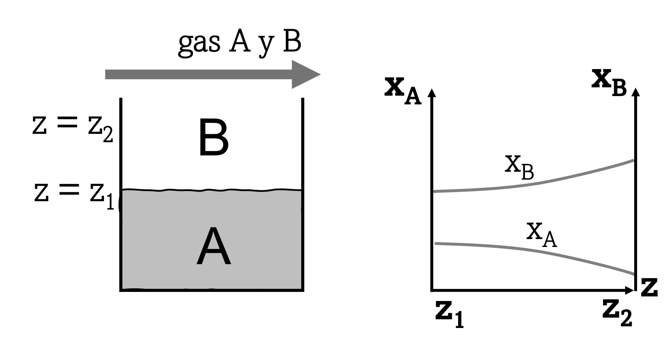
\includegraphics[scale=0.5]{./Capitulo2/Imagenes/fig-2-1.png}
	\caption{Columna de difusión. B no está en movimiento}
\end{figure}

A régimen permanente, la ec. (1.19) se reduce a:
\begin{equation}
\nabla \cdot \underline{N_A} = 0
\end{equation}

La ecuación (1.25) cuando $\underline{N_B} = 0$ se expresa como:

\begin{equation}
\underline{N_A} (1-x_A) = - c \mathcal{D}_{AB} \nabla x_A
\end{equation}

Si la difusión se da en una sola dirección (z), (2.1) y (2.2) requieren que:

\begin{equation}
	\frac{d}{dz} \left( \frac{c \mathcal{D}_{AB}}{1-x_A} \frac{dx_A}{dz} \right) = 0
\end{equation}

Integrando con respecto a z
$$
	\frac{1}{1-x_A} \frac{dx_A}{dz} = C_1
$$

Integrando de nuevo: 

\begin{equation}
- \ln{(1-x_A)} = C_1 z +C_2
\end{equation}

Condiciones de frontera 
\begin{equation}
	\left\{
	\begin{aligned}
	x_A |_{z=z_1} = x_{A1} \\
	x_A |_{z=z_2} = x_{A2}
	\end{aligned}
	\right.
\end{equation}

Se obtiene el siguiente perfil de concentraciones:

\begin{equation}
	\frac{1-x_A}{1-x_{A1}} = \left( \frac{1-x_{A2}}{1-x_{A1}} \right)^{\frac{z-z_1}{z_2-z_1}} 
	\qquad 
	1-x_A = x_B
\end{equation}

El flux de masa es:

\begin{equation}
N_{Az} |_{z=z_1} = \left. \frac{ - c \mathcal{D_{AB}}}{1-x_A} \frac{dx_A}{dz} \right|_{z=z_1} = \left. \frac{c \mathcal{D}_{AB}}{x_B} \frac{dx_B}{dz} \right|_{z=z_1} =  \frac{c \mathcal{D}_{AB}}{z_2 - z_1} \ln{\frac{x_{B2}}{x_{B1}}}
\end{equation}

que también puede ser expresado como: 

\begin{equation}
	N_{Az}|_{z=z_1} = \frac{c \mathcal{D}_{AB}}{(x_B)_{\ln{}}} \frac{(x_{A_1} - x_{A_2})}{z_2 - z_1}
\end{equation}

donde 

\begin{equation}
(x_B)_{\ln{}} = \frac{x_{B_2} - x_{B_1}}{\ln{(x_{B_2}/x_{B_1})}}
\end{equation}

En términos de las presiones, la ec. (2.8) se puede expresar: 

\begin{equation}
N_{Az}|_{z=z_1} = p \frac{\mathcal{D}_{AB}/RT}{z_2 - z_1} \ln{\left( \frac{p_{B_2}}{p_{B_1}}\right)} = p\frac{\mathcal{D}_{AB}/RT}{(p_B)_{\ln}} \frac{p_{A_1}-p_{A_2}}{z_2 - z_1}
\end{equation}


\subsection{Modelo de la película en transferencia de masa}

\begin{figure}[H]
	\centering
	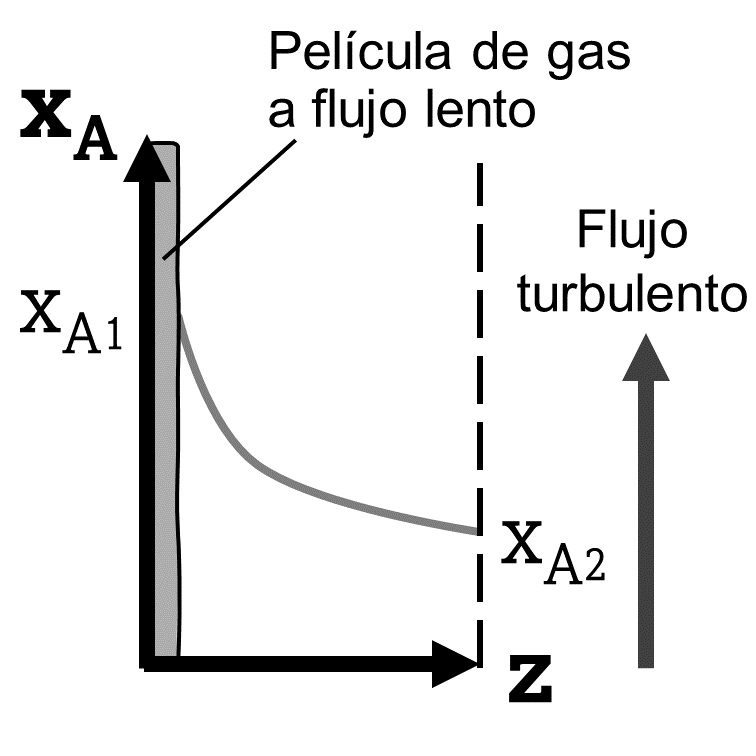
\includegraphics[scale=0.2]{./Capitulo2/Imagenes/fig-2-2.PNG}
	\caption{En este modelo, dentro de la película 		se produce la difusión de masa dentro de un 			medio a flujo lento.}
\end{figure}

\subsection{Difusión con interfase movible}

\begin{figure}[H]
	\centering
	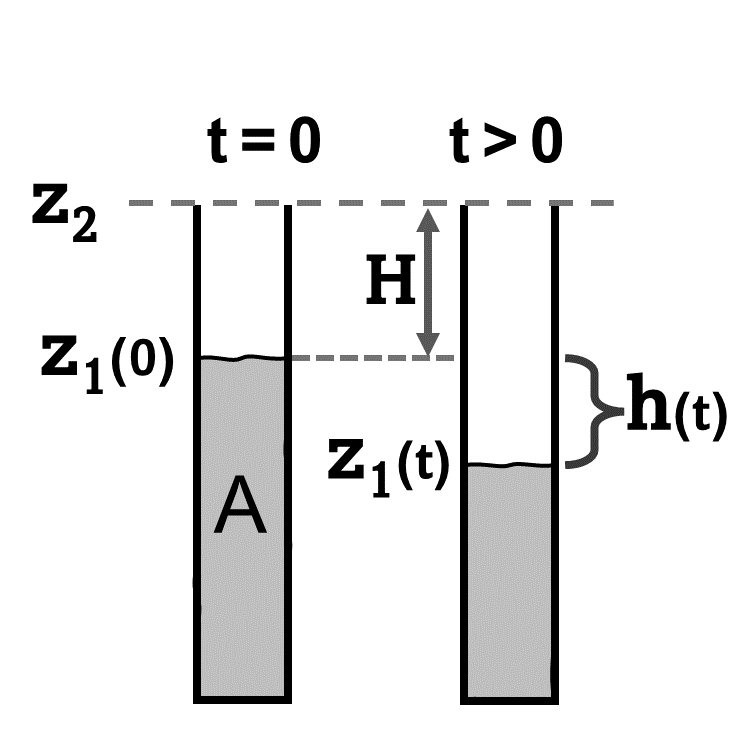
\includegraphics[scale=0.2]{./Capitulo2/Imagenes/fig-2-3.PNG}
	\caption{Evaporación con difusión cuasiestática. La mezcla de gases con concentración $x_{A_2}$ fluye arriba de los tubos.}
	\end{figure}
	
Primero, se iguala la velocidad de evaporación de $A$ con la velocidad a la que $A$ entra en la fase gas.

\begin{equation}
-\frac{p_A}{M_A} \frac{Sdz}{dt} = \frac{c \mathcal{D}_{AB}}{(x_B)_{\ln}} \frac{x_{A_1}-x_{A_2}}{z_2 - z_1} S
\end{equation}

Integrando la ec. (2.11): 

\begin{equation}
	\int_0^h (H+h)dh = \frac{c \mathcal{D}_{AB}}{(p_A/M_A)} \frac{(x_{A_1}-x_{A_2})}{(x_B)_{\ln}} \int_0^t dt = \frac{1}{2}c t
\end{equation}

en donde $h(t) = z_1(0) - z_1(t)$ y $H = z_2 - z_1(0)$ es la distancia inicial de la columna de gas. $c$ es una constante.

Integrando: 

\begin{equation}
	h(t) = H \left[ \sqrt{1+ct/H^2}-1 \right]
\end{equation}

Este experimento puede aportar la difusividad de mediciones del nivel del líquido como función del tiempo.

\subsection{Determinación de la difusividad}

La difusividad del par de gases $O_2 - CCl_4$ puede ser determinada por medio de datos de evaporación del $CCl_4$ en un tubo que contiene $O_2$ (ver figura 2.1). La distancia entre el nivel del $CCl_4$ líquido y la parte superior del tubo es $z_2 - z_1 = 17.1 \hspace{0.1cm} cm$. La presión total del sistema es $755 \hspace{0.1cm} mmHg$. y la temperatura es $0•^\circ C$. La presión de vapor del $CCl_4$ a $0•^\circ C$ es $33 \hspace{0.1cm} mmHg$. El área de sección del tubo es $0.82 \hspace{0.1cm} cm^2$. Se midieron $0.0208 \hspace{0.1cm} cm^3$ de $CCl_4$ evaporados en $10 \hspace{0.1cm} hrs$ en régimen permanente. ¿ Cuál es la difusividad del par $O_2 - CCl_4$ ?

\underline{Solución}:

Si $A=CCl_4$ y $B=O_2$. Entonces el flux molar de $A$ es:

$$N_A = \frac{\rho \text{Vol}}{M_A At} = \frac{(1.59)(0.0208)}{(154)(0.82)(36000)} = 7.26 \times 10­^{-9} gmol/cm^2 s$$ 

De la ec. (2.10):

$$N_{A_z} | _{z=z_1} = \frac{p}{RT} \mathcal{D}_{AB} \frac{\ln{(p_{B_2}/p_{B_1})}}{z_2 - z_1}$$

$$\mathcal{D}_{AB} = (7.2 \times 10^{-9})\frac{(17.1)}{\ln{(p_{B_2}/p_{B_1})}} \frac{RT}{p}$$

donde $R = 82.06 \hspace{0.1cm} \frac{cm^3 atm}{gmol K}$, $T = 273 \hspace{0.1cm} K$

$$p = \frac{755}{760} \hspace{0.1cm} atm , \hspace{0.5cm} \frac{p_{B_2}}{p_{B_1}} = \frac{755}{755-33}$$

$$\mathcal{D}_{AB} = 0.0636 \hspace{0.1cm} cm^2/s$$
	
\section{Difusión-Convección de masa}

\subsection{Convección forzada. Absorción de gas $A$ en una película descendente de líquido $B$}

\begin{figure}[H]
	\centering
	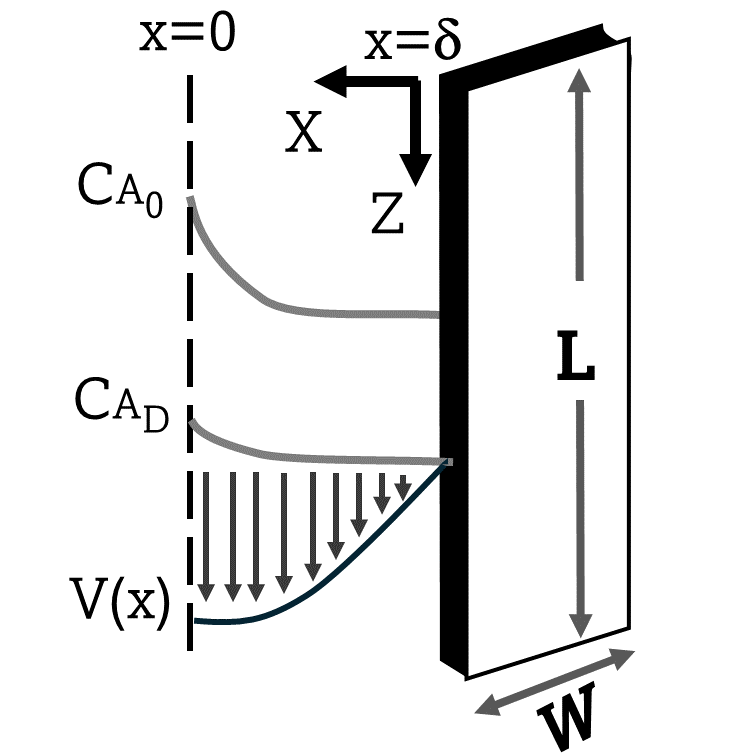
\includegraphics[scale=0.2]{./Capitulo2/Imagenes/fig-2-4.PNG}
	\caption{Absorción de $A$ en una película descendente de líquido $B$.}
\end{figure}

El perfil de velocidades en una solución diluida (la viscosidad es la del solvente) es:

\begin{equation}
v_z(x) = v_{\text{máx}} \left( 1 - \frac{x^2}{\delta^2} \right)
\end{equation}

Si el perfil de concentraciones se da en la zona de velocidad máxima, se puede considerar una velocidad constante $v_{\text{máx}}$. Un ejemplo es la absorción de $O_2$ en $H_2O$.

Debido a que $C_A = C_A(x,z)$, existen dos fluxes $N_{Ax}$ y $N_{Az}$. La ec. (2.1) a régimen permanente y sin reacción química se reduce a:

\begin{equation}
	\nabla \cdot \underline{N_A} = 0 \to \frac{\partial N_{Ax}}{\partial x} + \frac{\partial N_{Az}}{\partial z} = 0
\end{equation}

A partir de la ec. (1.30) se obtiene:

%\begin{equation}%
%Use \label{original} and \tag{\ref{eq:original}}%
$$	\underline{v} \cdot \nabla C_A = \mathcal{D}_{AB} \nabla^2 C_A $$
%\end{equation}%

que para $\underline{v} = (0, 0, v_z)$ tenemos:

\begin{equation} \label{eq: manrefx}
	v_z \frac{\partial C_A}{\partial z} = \mathcal{D}_{AB} \left[ \frac{\partial^2 C_A}{\partial x^2} + \frac{\partial^2 C_A}{\partial z^2}  \right]
\end{equation}

Definiendo al número de Peclet de masa ($Pe_M$) como: 

\begin{equation}
	Pe_M = Re Sch = \frac{uL}{\nu} \cdot \frac{\nu}{\mathcal{D}_{AB}} = \frac{uL}{\mathcal{D}_{AB}}
\end{equation}

donde $u$ y $L$ son la velocidad y longitud características. En este caso $u = v_{\text{máx}}$. Se supone que a lo largo del eje $z$:

$$Pe_M = \frac{v_{\text{máx}} L}{\mathcal{D}_{AB}} > 1$$

El término convectivo predomina sobre el difusivo, por lo que

$$v_z \frac{\partial C_A}{\partial z} > \mathcal{D}_{AB} \frac{\partial^2 C_A}{\partial z^2}$$

y la ec. \eqref{eq: manrefx} se simplifica:

\begin{equation} \label{eq: manrefx2}
v_{z \text{máx}} \frac{\partial C_A}{\partial z} = \mathcal{D}_{AB} \frac{\partial^2 C_A}{\partial x^2}
\end{equation}

Como $dt = \frac{dz}{v_{\text{máx}}}$, entonces la ec. \eqref{eq: manrefx2} se expresa como:

\begin{equation} \label{eq: manrefx3}
	\frac{\partial C_A}{\partial t} = \mathcal{D}_{AB} \frac{\partial^2 C_A}{\partial x^2}
\end{equation}

Las condiciones de frontera son:

\begin{equation}
	\text{Condición inicial:} \hspace{0.5cm} C_A|_{z=0} = 0 \hspace{0.5cm} \text{($B$ puro)}
\end{equation}

\begin{equation}
	 \text{Condición de interfase:} \hspace{0.4cm} C_A|_{x=0} = C_{A0} \hspace{0.4cm} \text{(Solubilidad de $A$ en $B$)}
\end{equation}

La condición $\left. \frac{\partial C_A}{\partial x} \right|_{x = \delta} = 0$ (flujo de masa es cero en la pared) se cambia por:

\begin{equation}
	C_A|_{x \to \infty} = 0
\end{equation}

(el perfil de $C_A$ se encuentra cerca de la interfase y lejos de la pared)

Considerando la concentración de $C_A$ adimensional:

\begin{equation}
	C_A' = \frac{C_A}{C_{A0}}
\end{equation}

La solución de \eqref{eq: manrefx3} se obtiene por el método de combinación de variables, que consiste en formar un grupo adimensional con las variables de la ecuación. Se sugiere la siguiente relación:

\begin{equation}
	C_A' = C_A'(\eta) \hspace{0.5cm} \text{donde} \hspace{0.5cm} \eta = \frac{x}{\sqrt{4 \mathcal{D}_{AB} t}}
\end{equation}

de tal forma que:

\begin{equation} \label{eq: manrefx4}
	\frac{d C_A'}{dt} = \frac{d C_A'}{d \eta} \frac{\partial \eta}{\partial t} = \frac{x}{\sqrt{4 \mathcal{D}_{AB}}} \left( - \frac{1}{2} t^{-3/2}  \right) = - \frac{1}{2} \frac{\eta}{t} \frac{d C_A'}{d \eta}
\end{equation}

$$\frac{dC_A'}{dx} = \frac{dC_A'}{d \eta} \frac{\partial \eta}{\partial x} = \frac{1}{\sqrt{4 \mathcal{D}_{AB} t}} \frac{dC_A'}{d \eta}$$

\begin{equation} \label{eq: manrefx5}
	\frac{\partial^2 C_A'}{\partial x^2} =  \frac{d^2 C_A'}{d \eta^2} \frac{1}{4 \mathcal{D}_{AB}t}
\end{equation}

Sustituyendo \eqref{eq: manrefx4} y \eqref{eq: manrefx5} en la ec. \eqref{eq: manrefx3} se obtiene: 

\begin{equation} \label{eq: manrefx6}
	\frac{d^2 C_A'}{d \eta^2} + 2\eta \frac{d C_A'}{d \eta} = 0
\end{equation}

Condiciones de frontera:

\begin{equation} \label{eq: manrefx7}
	C_A'|_{\eta = 0} = 1
\end{equation}

\begin{equation} \label{eq: manrefx8}
	C_A'|_{\eta \to \infty} = 0
\end{equation}

La primera integración de la ec. \eqref{eq: manrefx6} da:

Si $\frac{d C_A'}{d \eta} = \phi \to \frac{d\phi}{d \eta} + 2 \eta \phi = 0 \to \ln{\phi} = -\eta^2 + \ln{C_1}$

\begin{equation} \label{eq: manrefx8.1}
	\frac{dC_A'}{d \eta} = C_1 e^{-\eta^2}
\end{equation}

La segunda integración da por resultado:

\begin{equation} \label{eq: manrefx9}
	C_A' = C_1 \int_0^\eta e^{-\bar{\eta}^2} d\bar{\eta} + C_2
\end{equation}

La condición \eqref{eq: manrefx7} implica que $C_2 = 1$. La condición \eqref{eq: manrefx8} nos da:

$$0 = C_1 \int_0^\infty e^{-\bar{\eta}^2} d\bar{\eta} +1 = C_1 \frac{\sqrt{\pi}}{2} + 1 \to C_1 = \frac{-2}{\sqrt{\pi}}$$

Sustituyendo $C_1$ y $C_2$ en la ec. \eqref{eq: manrefx9} obtenemos: 

\begin{equation}
C_A' = 1 - \frac{2}{\sqrt{\pi}} \int_0^\eta e^{-\bar{\eta}^2} d\bar{\eta} = 1 - \text{erf} (\eta) = \text{erfc}(\eta) 
\tag{\ref{eq: manrefx8.1}}
\end{equation}

 donde $\text{erf} (\eta)$ es la función error y $\text{erfc}(\eta)$ es la función complementaria (ver fig. 2.5).
 
 \begin{figure}[H]
 	\centering
 	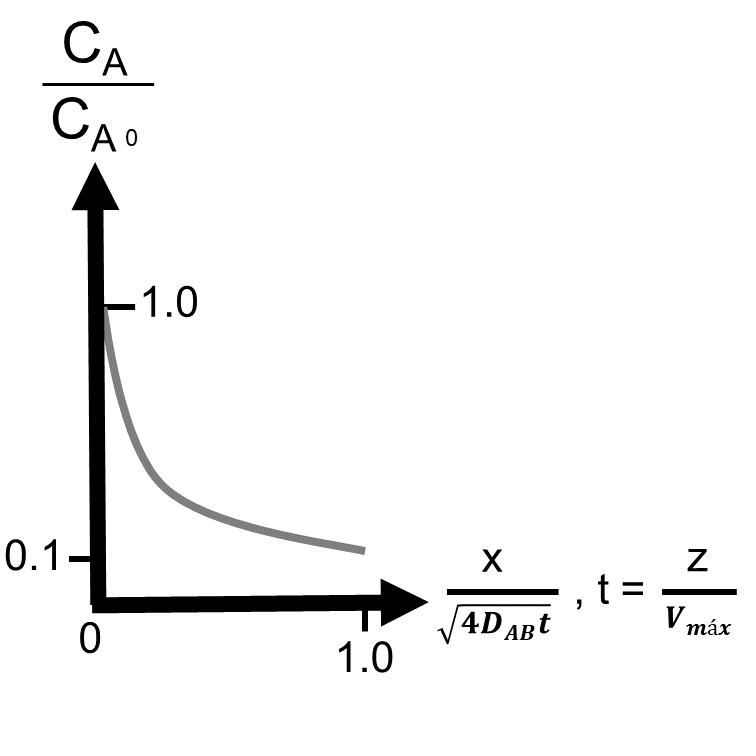
\includegraphics[scale=0.3]{./Capitulo2/Imagenes/fig-2-5.PNG}
 	\caption{Perfil de concentraciones donde $\delta$ es la longitud característica para la difusión de A en B.}
 \end{figure}
 
 Cuando $\eta = 2$, $\frac{C_A}{C_{A0}} \sim 0.01$ se puede definir una capa límite de difusión de $A$ en $B$ $\frac{\delta}{\sqrt{4\mathcal{D}_{AB}t}} = 2 \to \delta = 4 \sqrt{\mathcal{D}_{AB}t}$
 
 El flux de masa local en la interfase se puede obtener:
 
 $$N_{Ax}|_{x=0} = -\mathcal{D}_{AB} \left. \frac{\partial C_A}{\partial x} \right|_{x=0} = -\mathcal{D}_{AB} C_{A0} \left. \frac{\partial C_A'}{\partial \eta} \right| _{\eta = 0} \frac{\partial \eta}{\partial x} = -\mathcal{D}_{AB} \left( \frac{-2}{\sqrt{\pi}} \right) \frac{C_{A0}}{\sqrt{\mathcal{D}_{AB}t}}$$
 
 \begin{equation}
 	N_{Ax}|_{x=0} = C_{A0} \sqrt{\frac{\mathcal{D}_{AB}t}{\pi}} = C_{A0} \sqrt{ \frac{\mathcal{D}_{AB} v_{\text{máx}}}{\pi z}}
 	\tag{\ref{eq: manrefx9}}
 \end{equation}
 
 El flujo de masa de $A$ absorbido por $B$ es la superficie $LW$ es:
 
 $$W_A = \int_0^W \int_0^L N_{Ax}|_{x=0} dz dy = WC_{A0} \sqrt{\frac{\mathcal{D}_{AB} v_{\text{máx}}}{\pi}} \int_0^L \frac{dz}{\sqrt{z}}$$
 
 \begin{equation} \label{eq: manrefx10}
 W_A = WLC_{A0} \sqrt{\frac{4\mathcal{D}_{AB} v_{\text{máx}}}{\pi L}}
 \end{equation}
 
 Este desarrollo se puede aplicar a la absorción de gas en burbujas ascendentes.
 
 \begin{figure}[H]
 	\centering
 	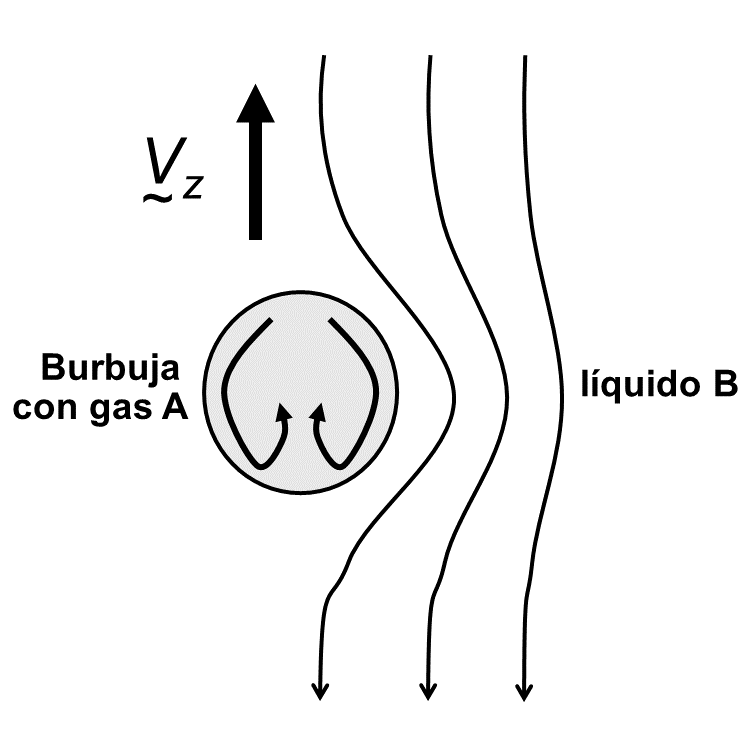
\includegraphics[scale=0.2]{./Capitulo2/Imagenes/fig-2-6.PNG}
 	\caption{Burbuja de gas $A$ ascendiendo en un líquido $B$ a velocidad $\underline{v_t}$.}
 \end{figure}
 
 Se puede utilizar la ec. \eqref{eq: manrefx10} para calcular la absorción de gas, reemplazando el tiempo de contacto 
 
 $$t_{\text{exp}} = \frac{L}{v_{\text{máx}}} = \frac{D}{v_t} \frac{\text{(diámetro de la burbuja)}}{\text{(velocidad de la burbuja)}}$$
 
 Si $C_{A0}$ es la solubilidad de A en B, la rapidez de absorción molar es:
 
 \begin{equation}
 	(N_A)_{\text{prom}} = C_{A0} \sqrt{\frac{4 \mathcal{D}_{AB} v_t}{\pi D}}
 \end{equation}
 
\subsection{Disolución de sólidos en una película descendente}

\begin{figure}[H]
	\centering
	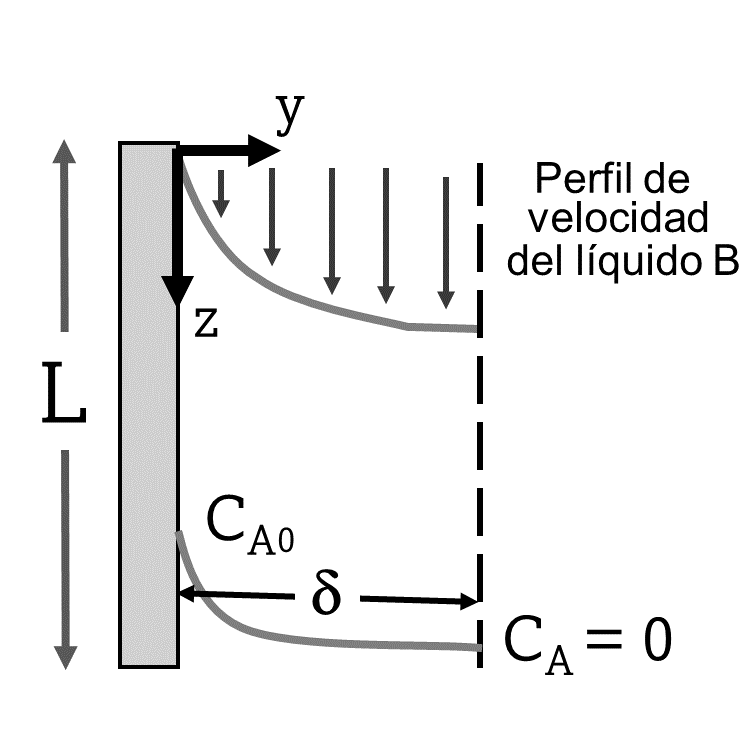
\includegraphics[scale=0.2]{./Capitulo2/Imagenes/fig-2-7.PNG}
	\caption{El sólido $A$ se disuelve en el líquido $B$ que desciende.}
\end{figure}

La concentración de $A$ en el líquido $B$ cambia dentro de una capa límite junto al sólido. El perfil de velocidades en una película descendente vertical, es:

\begin{equation}
	v_z = \frac{\rho g \delta^2}{2 \mu} \left[ 1 - \left( \frac{y'}{\delta} \right)^2 \right]
\end{equation}

En la aproximación de capa límite, se puede linealizar el perfil cerca de la pared, definiendo una variable $y$ de la forma: $y = \delta - y'$, de tal forma que: $1- \left( \frac{y'}{\delta} \right)^2 = 1 - \left( \frac{\delta - y}{\delta} \right)^2 = 1 - \left( 1- 2 \frac{y}{\delta} \right) =  \frac{2y}{\delta}$.  El perfil resultante es:

\begin{equation}
	v_z = \left( \frac{\rho g \delta}{\mu} \right) y = ay
\end{equation}

La ecuación de difusión en este caso es:

\begin{equation} \label{eq: manrefx10.1}
	ay \frac{\partial C_A}{\partial z} = \mathcal{D}_{AB} \frac{\partial^2 C_A}{\partial y^2}
\end{equation}

Las condiciones de frontera son:

\begin{equation}
	C_A|_{z=0} = 0
\end{equation}

\begin{equation}
	C_A|_{y=0} = C_{A0}
\end{equation}

\begin{equation}
	C_A|_{y \to \infty} = 0 \hspace{0.5cm} \text{(tiempo de contacto corto)}
\end{equation}

Por el método de combinación de variables, se sugiere la siguiente combinación:

\begin{equation} \label{eq: manrefx11}
	\frac{C_A}{C_{A0}} = f(\eta) \hspace{0.5cm} \text{donde} \hspace{0.5cm} \eta = y \left( \frac{a}{9 \mathcal{D}_{AB}z} \right)^{1/3}
\end{equation}

\begin{equation}
	\frac{\partial f}{\partial z} = \frac{\partial f}{\partial \eta} \left( \frac{\partial \eta}{\partial z} \right) = - y \left( \frac{a}{9 \mathcal{D}_{AB}} \right)^{1/3} \left( - \frac{1}{3} \frac{z^{-1/3}}{z} \right) = - \frac{1}{3} \frac{\eta}{z} \frac{d f}{d \eta}
\end{equation}

$$
\frac{\partial f}{\partial y} = \frac{\eta}{y} \frac{df}{d\eta} = \left( \frac{\partial \eta}{\partial y} \right) \frac{d f}{d \eta}
$$

\begin{equation} \label{eq: manrefx12}
	\frac{\partial^2 f}{\partial y^2} = \frac{\eta}{y} \frac{\partial \eta}{\partial y} \frac{d^2 f}{d y^2} = \frac{\eta^2}{y^2} \left( \frac{d^2 f}{d \eta^2} \right)
\end{equation}

Sustituyendo \eqref{eq: manrefx11} y \eqref{eq: manrefx12} en la ec. \eqref{eq: manrefx10.1} resulta en:

\begin{equation} \label{eq: manrefx13}
	\frac{d^2 f}{d \eta^2} + 3 \eta^2 \frac{df}{d \eta} = 0
\end{equation}

con condiciones de frontera:

\begin{equation} \label{eq: manrefx14}
	f|_{\eta = 0} = 1
\end{equation}

\begin{equation} \label{eq: manrefx15}
	f|_{\eta \to \infty} = 0
\end{equation}

La solución de \eqref{eq: manrefx13} es:

\begin{equation} \label{eq: manrefx16}
	f = C_1 \int_0^\eta e^{-\bar{\eta}^3} d \bar{\eta} + C_2
\end{equation}

La condición \eqref{eq: manrefx14} determina $C_2 = 1$. La condición \eqref{eq: manrefx15} determina \\ $C_1 = \dfrac{-1}{\int_0^\infty e^{-\bar{\eta}^3} d \bar{\eta}} = - \frac{1}{\Gamma (\frac{4}{3})}$ 

donde $\Gamma (x)$ es la función gamma de x. Como $\int_0^\eta = \int_0^\infty - \int_\eta^\infty$ entonces:

\begin{equation} \label{eq: manrefx16.1}
	\frac{C_A}{C_{A0}} = f =  \frac{\int_\eta^\infty e^{-\bar{\eta}^3} d\bar{\eta}}{\Gamma(\frac{4}{3})}
	\tag{\ref{eq: manrefx16}}
\end{equation}

\begin{equation}
	\begin{split}
	N_{Ay}|_{y=0} = - \mathcal{D}_{AB} \left.  \frac{\partial C_A}{\partial y} \right|_{y=0} = - \mathcal{D}_{AB} C_{A0} \left[ \frac{d}{d\eta} \left( \frac{C_A}{C_{A0}} \right) \frac{\partial \eta}{\partial y} \right]_{y=0} 
	\\
  = -\mathcal{D}_{AB} C_{A0} \left[ \frac{- e^{-\eta^3}}{\Gamma(\frac{4}{3})} \left( \frac{a}{9 \mathcal{D}_{AB}z} \right)^{1/3} \right]_{y=0} = \frac{\mathcal{D}_{AB} C_{A0}}{\Gamma (\frac{4}{3})} \left( \frac{a}{9 \mathcal{D}_{AB} z} \right)^{1/3}
	\end{split}
\end{equation}

El flujo molar de $A$ en $y=0$ es:

\begin{equation}
	\begin{split}
	W_A = \int_0^W \int_0^L N_{Ay}|_{y=0} dz dx
	=W \frac{\mathcal{D}_{AB} C_{A0}}{\Gamma(\frac{4}{3})} \left( \frac{a}{9 \mathcal{D}_{AB}} \right)^{1/3} \int_0^L z^{-1/3} dz \\
	=\left( \frac{3}{2} \right) \frac{\mathcal{D}_{AB} C_{A0} W}{\Gamma (\frac{4}{3})} \left( \frac{a}{9 \mathcal{D}_{AB}} \right)^{1/3} L^{2/3}
	=\frac{2 \mathcal{D}_{AB} C_{A0} WL}{\frac{4}{3} \Gamma (\frac{4}{3})} \left( \frac{a}{9 \mathcal{D}_{AB} L} \right)^{1/3}
	\end{split}
\end{equation}

donde $\frac{4}{3} \Gamma (\frac{4}{3}) = \Gamma (\frac{7}{3})$

\subsection{Perfil de concentración en un reactor tubular}

\begin{figure}[H]
	\centering
	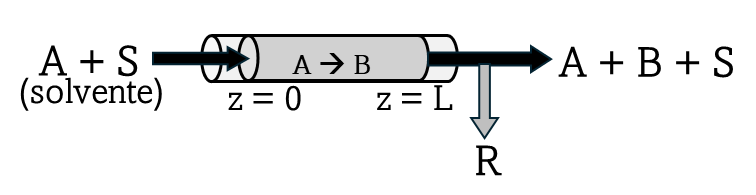
\includegraphics[scale=0.4]{./Capitulo2/Imagenes/fig-2-8.PNG}
	\caption{Reactor tubular}
\end{figure}

La situación es similar a las condiciones de la ec. \eqref{eq: manrefx2} en coordenadas cilíndricas, esto es: 

\begin{equation} \label{eq: manrefx17}
v_z \frac{\partial C_A}{\partial z} = \mathcal{D}_{AB} \left[ \frac{1}{r} \frac{\partial}{\partial r} \left( r \frac{\partial C_A}{\partial r} \right)  \right]
\end{equation}

\begin{equation} \label{eq: manrefx18}
\text{donde} \hspace{0.5cm} v_z = v_{z\text{máx}} \left[ 1 - \left( \frac{r}{R} \right)^2 \right]
\end{equation}

con condiciones:

\begin{equation}
C_A|_{z=0} = C_{A0} \hspace{0.2cm} , \hspace{0.2cm} C_A|_{r=R} = 0 \hspace{0.2cm} \text{y} \hspace{0.2cm} C_A|_{r=0} \neq 0
\end{equation}

La linealización del perfil de velocidades cerca de la pared procede definiendo una variable $y = R-r$:

Como $v_{\text{máx}} = \frac{\Delta P R^2}{2 \mu L}$, entonces $v_z (y) = v_{\text{máx}} \frac{y}{R} $

La ec. \eqref{eq: manrefx17} se transforma en:

\begin{equation}
	2 v_{\text{máx}} \frac{y}{R} = \mathcal{D}_{AB} \frac{\partial^2 C_A}{\partial y^2}
\end{equation}

debido a que $\frac{y}{R} = 1 - \frac{r}{R}$, entonces $\left( \frac{r}{R} \right)^2 = \left( 1 - \frac{y}{R} \right)^2 \approx 1 - \frac{2 y}{R} + \cdots$ por lo que $v_z = v_{z \text{máx}} (\frac{2y}{R})$ (ec. \eqref{eq: manrefx18}) con nuevas condiciones:

\begin{equation}
C_A|_{z=0} = C_{A0} \hspace{0.2cm} , \hspace{0.2cm} C_A|_{y=0} = 0 \hspace{0.2cm} \text{y} \hspace{0.2cm} C_A|_{y \to \infty} = C_{A0}
\end{equation}

La solución es similar a la ec. \eqref{eq: manrefx16.1}, excepto que ahora $f|_{\eta = 0} = 0$ y \\ $f|_{\eta \to \infty} = 1$. Las constantes son: $C_2 = 0$ y $C_1$ es igual: $C_1 = \frac{-1}{\Gamma (\frac{4}{3})}$, por lo tanto:

\begin{equation}
	\frac{C_A}{C_{A0}} = \frac{\int_0^\eta e^{- \bar{\eta}^3} d \bar{\eta}}{\Gamma (\frac{4}{3})}
\end{equation}


\section{Difusión con reacción química homogénea}

\begin{minipage}{0.5\textwidth} 
    \centering
    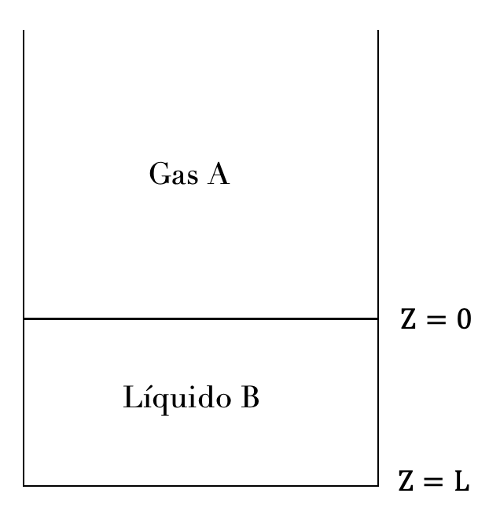
\includegraphics[width=0.8\linewidth]{Capitulo2/Imagenes/Fig_2.9.png} 
    \captionof{figure}{Absorción de A en B con reacción homogénea en la fase líquida} 
    \label{fig:Fig_2.9}
\end{minipage}%
\begin{minipage}{0.4\textwidth} 
    En la figura \textbf{\eqref{fig:Fig_2.9}}, el gas \( A \) se disuelve en el líquido \( B \). Al difundirse \( A \) en \( B \), ocurre una reacción \( A + B \xrightarrow{} AB \). Por ejemplo, la absorción de \( CO_2 \) en una solución de NaOH.
        En este caso, el proceso es descrito por la ecuación \textbf{\eqref{eq_1.30}}, en la cual, no hay dependencia con el tiempo y el sistema está en reposo \( \underline{v} = 0 \).
\end{minipage}
    

\vspace{1 cm}
Suponiendo una reacción de primer orden para la descomposición de A, la ecuación \textbf{\eqref{eq_1.30}} se reduce a:

\begin{equation}   
 \mathscr{D}_{AB}\frac{d^2(C_A)}{dz^2}+R_A=0
 \label{eq_2.55}
\end{equation}


En donde:\begin{equation}
    R_A=\frac{d(C_A)}{dt}=-kC_A
    \label{eq_2.56}
\end{equation}
Este sistema otorga las siguientes condiciones de frontera:

\begin{equation}
    C_A|_{z=0} = C_{A0}, \quad \frac{d(C_A)}{dz}\bigg|_{z=L} = N_{Az}|_{z=L} = 0
    \label{eq_2.57}
\end{equation}

Se definen las siguientes variables adimensionales: $\Gamma=\frac{C_A}{C_{A0}}$ y $\zeta=\frac{z}{L}$

La ecuación \eqref{eq_2.55} se transforma en:
\begin{equation}
    \frac{d^2\Gamma}{d\zeta^2}-\left(\frac{k_1L^2}{\mathscr{D}_{AB}}\right)\Gamma=0
    \label{eq_2.58}
\end{equation}
\quad donde
\begin{equation}
  \phi=\left( \frac{k_1L^2}{\mathscr{D}_{AB}}\right)^{1/2}
\end{equation}

es el módulo de Thiele. \\Las condiciones de frontera adimensionales son ahora:
\begin{equation}
 \Gamma|_{\zeta=0}=1   
\quad \text{y} \quad
 \frac{d\Gamma}{d\zeta}|_{\zeta=1}=0   
 \label{eq_2.60}
\end{equation}

La solución de la ecuación \eqref{eq_2.58} corresponde a:
\begin{equation}
    \Gamma=C_1\cosh({\phi\zeta})+C_2\sinh({\phi\zeta})
    \label{eq_2.61}
\end{equation}
Aplicando \eqref{eq_2.61} obtenemos $C_1$ y $C_2$:

 $C_1=1$ y $0=\phi \sinh({\phi})+C_2\phi \cosh(\phi)\longrightarrow C_2=-\frac{\sinh(\phi)}{\cosh({\phi})}=-\tanh({\phi})$
La ec. \eqref{eq_2.60} tiene la siguiente solución particular:
 \begin{equation}
  \Gamma=\frac{\cosh[{\phi(1-\zeta)}]}{\cosh({\phi})}   
  \label{eq_2.62}
 \end{equation}

La concentración promedio de A en la fase líquida es;

 \begin{equation}
     \overline{\Gamma}=\frac{\int_0^1\Gamma d\zeta}{\int_0^1d\zeta}=\frac{1}{\cosh(\phi)}\left[\frac{\sinh[\phi(1-\zeta)]_{0}^1}{-\phi}\right]=\frac{\tanh(\phi)}{\phi}
     \label{eq_2.63}
 \end{equation}
 
El flux molar en $z=0$ es:

\begin{equation}
    N_{Az}|_{z=0}=-\mathscr{D}_{AB}\frac{d(C_A)}{dz}|_{z=0}=-\mathscr{D}_{AB}\frac{C_{A0}}{L}\frac{d\Gamma}{d\zeta}|_{\zeta=0}=\mathscr{D}_{AB}\frac{C_{A0}}{L}\phi\tanh(\phi)
\end{equation}



\subsection{Absorción de gas con reacción química en un tanque de agitación}
Considere un sistema en el que el gas A disuelto se combina con el líquido B por una reacción química de primer orden. Por ejemplo, la absorsión de $SO_2$ o $H_2S$ en NaOH en solución acuosa.

\begin{figure}[H]
    \centering
    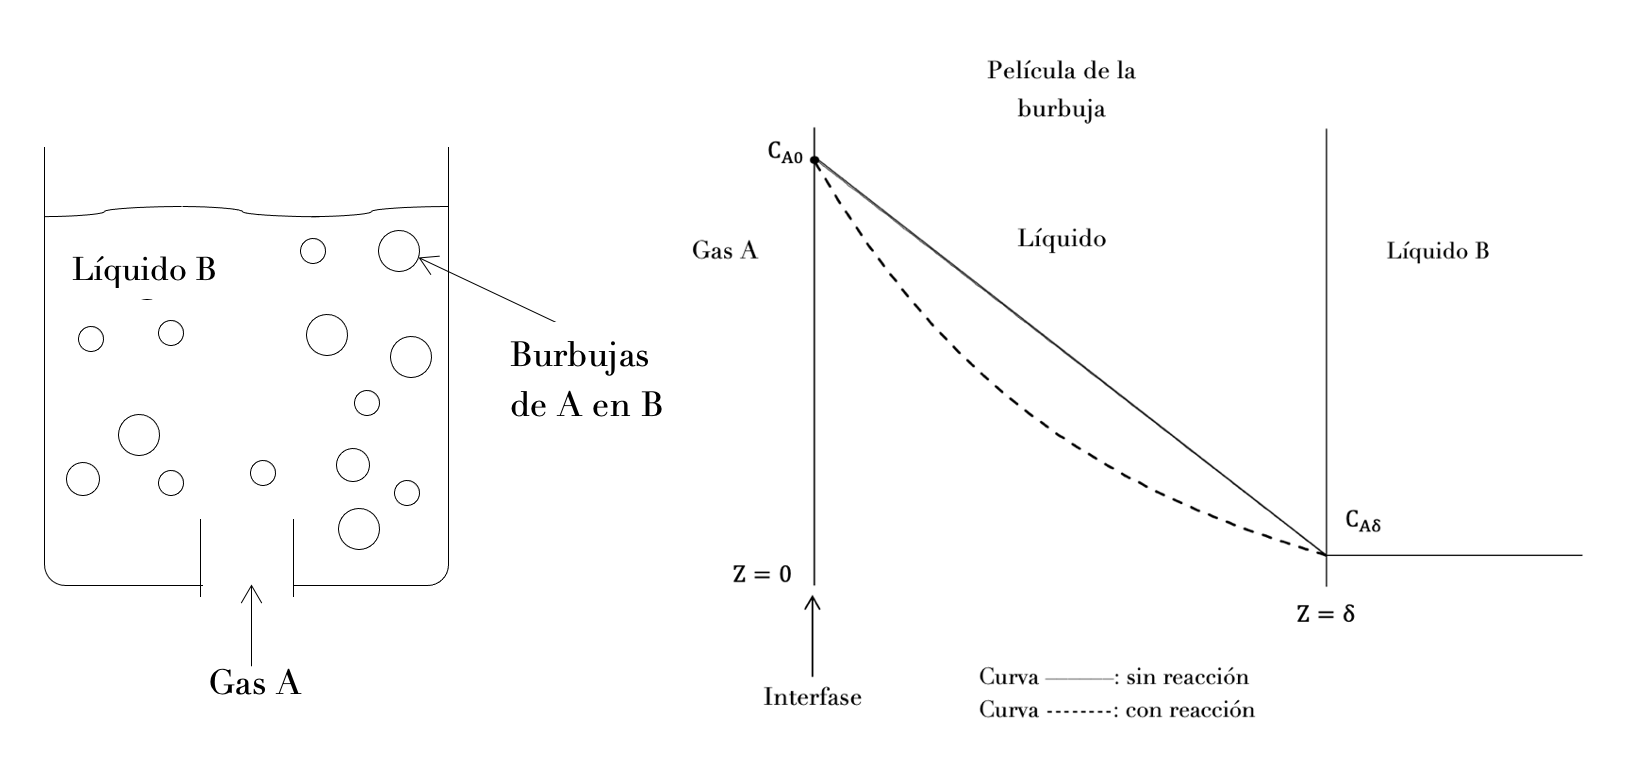
\includegraphics[width=\linewidth]{Capitulo2/Imagenes/Fig_2.10.png}
    \caption{Perfil de concentración predicho en la película de líquido que rodea a una burbuja}
    \label{fig:fig_2.10}
\end{figure}

Condiciones de forntera:
\begin{equation}
    C_A|_{z=0}=C_{A0} \quad\text{y}\quad
    C_A|_{z=\delta}=C_{A\delta}
\end{equation}
O en variables adimensionales:
\begin{equation}
    \Gamma|_{\zeta=0}=1 \quad \text{y} \quad
    \Gamma|_{\zeta=1}=B
        \label{eq_2.66}
\end{equation}
En donde 
\begin{equation*}
    \zeta = \frac{z}{\delta}, \quad \Gamma = \frac{C_A}{C_{A0}}, \quad B = \frac{C_{A\delta}}{C_{A0}}, \quad \phi^2 = \frac{k_1 \delta^2}{\mathscr{D}_{AB}}
\end{equation*}


La ecuación \eqref{eq_2.61} con las condiciones \eqref{eq_2.66} tiene la siguiente solución:

\begin{equation}
    \Gamma=\frac{\sinh(\phi)\cosh(\phi\zeta)+(B-\cosh(\phi))\sinh(\phi\zeta)}{\sinh(\phi)}
    \label{eq_2.67}
\end{equation}
La ecuación \eqref{eq_2.67} describe el perfil de la curva con reacción. Se supone que la concentración de A fuera de la película es $C_{A\delta}$, por lo que, si la superficie de todas las burbujas en la superficie es S, la cantidad de A consumida por la reacción química es:

\begin{equation}
    SN_{Az}|_{z=\delta}=-S\mathscr{D}_{AB}\frac{dC_A}{dz}|_{z=\delta}=Vk_1C_A\delta
    \label{eq_2.68}
\end{equation}
En donde V es el volumen de la fase líquida.
Luego:

\begin{equation*}
    -\frac{dC_A}{dz}|_{z=\delta}=-\frac{C_{A0}}{\delta}\frac{d\Gamma}{d\zeta}|_{\zeta=1}=\frac{Vk_1C_{A\delta}}{S\mathscr{D}_{AB}}\longrightarrow-\frac{d\Gamma}{d\zeta}|_{\zeta=1}=\frac{V}{S\delta}\phi^2B
\end{equation*}
Como $\cosh^2(\phi)-\sinh^2(\phi)=1$, de la ec. \eqref{eq_2.67} se obtiene:

\begin{equation*}
    \frac{B\cosh(\phi)-1}{\sinh(\phi)}=-\frac{V}{S\delta}B\phi\longrightarrow B(\cosh(\phi)+\frac{V}{S\delta}\phi\sinh(\phi))=1
\end{equation*}
Substituyendo B en la solución para Gamma \eqref{eq_2.67}, obtenemos:
\begin{equation}
    \Gamma=\frac{\cosh(\phi)\cosh(\phi\zeta)-\cosh(\phi)\sinh(\phi\zeta)}{\sinh(\phi)}+\frac{\sinh(\phi)\zeta}{\sinh(\phi)}[\frac{1}{\cosh(\phi)+\frac{V\phi\sinh(\phi)}{S\delta}}]
    \label{eq_2.69}
\end{equation}
El flux de masa absorbido con reacción química ( normalizada) es:

\begin{equation}
\begin{split}
    \widetilde{N} &= \frac{N_{Az}}{\mathscr{D}_{AB}\frac{C_{A0}}{\delta}} = -\frac{\mathscr{D}_{AB}}{\mathscr{D}_{AB}\frac{C_{A0}}{\delta}} \frac{d(C_A)}{dz}\bigg|_{z=0} \\
    &\Rightarrow -\frac{d\Gamma}{d\zeta}\bigg|_{\zeta=0} = \frac{\phi \cosh(\phi)}{\sinh(\phi)} - \frac{\phi}{\sinh(\phi)\left(\cosh(\phi) + \frac{V\phi \sinh(\phi)}{S\delta}\right)} \\
    &= \frac{\phi}{\sinh(\phi)}\left[\cosh(\phi) - \frac{1}{\cosh(\phi) + \frac{V}{S\delta}\phi \sinh{\phi}}\right]
\end{split}
\label{eq_2.70}
\end{equation}

\begin{figure}[H]
    \centering
    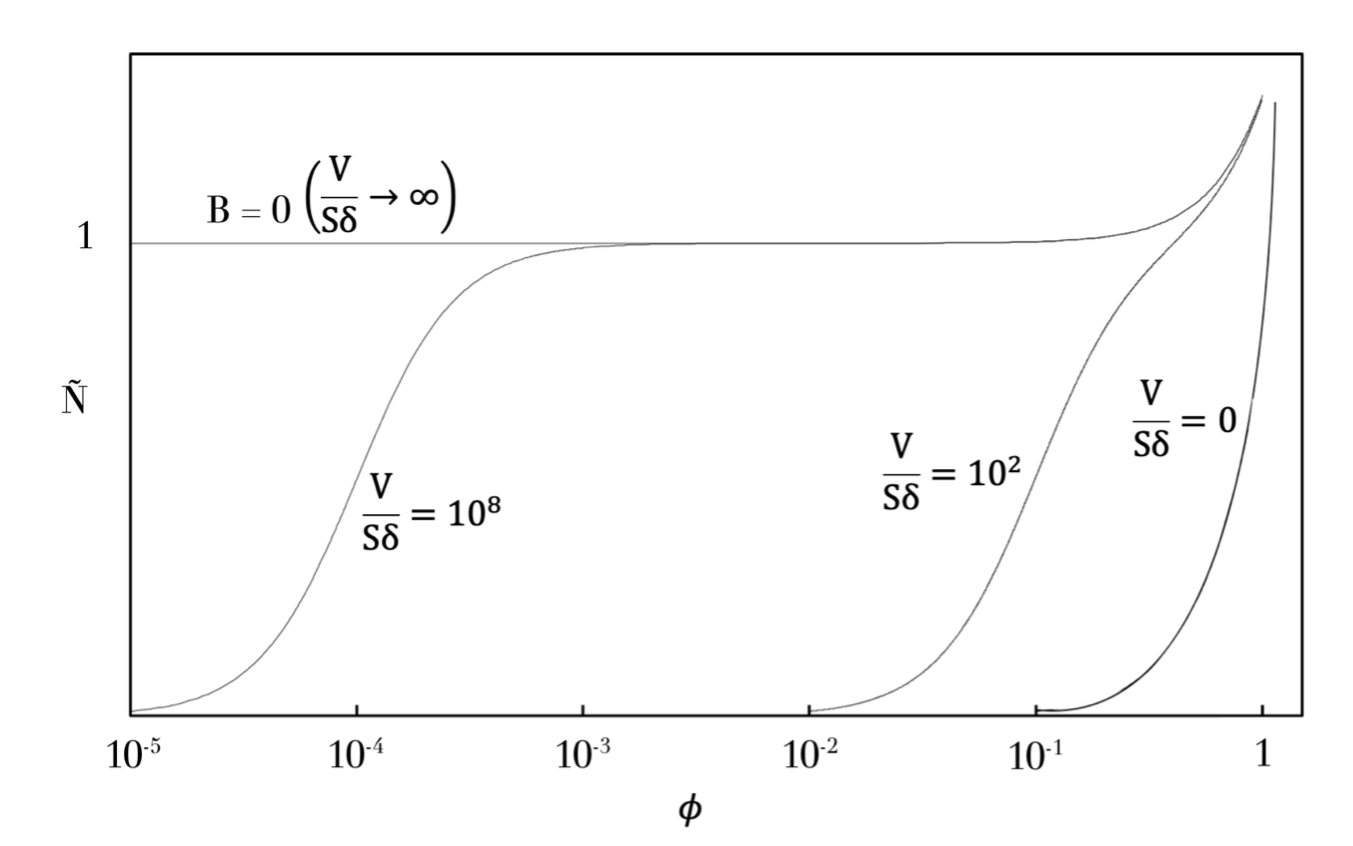
\includegraphics[width=\linewidth]{Capitulo2/Imagenes/Imagen_11_cap_2.png}
    \caption{Absorición de gas con reacción química}
    \label{fig:fig_2.11}
\end{figure}

La ecuación \eqref{eq_2.70} se grafica en la fig. \eqref{fig:fig_2.11}. Se puede observar en la fig. \eqref{fig:fig_2.11}:
\begin{enumerate}
    \item $\widetilde{N}$ aumenta con $\phi$ para todo $\frac{V}{S\delta}$
    \item $\widetilde{N}=1$ es la curva sin reacción que corresponde a la \eqref{fig:fig_2.10}. Cuando $\phi=0$ $\widetilde{N}\rightarrow1$ ($B=0$)
    \item Cuando $\phi\rightarrow0$, para $\frac{V}{S\delta}$ finito $\widetilde{N}=0$, se lidia con un líquido saturado con gas disuelto.
    \item Si $\phi$ es grande, $\widetilde{N}$ se incrementa abruptamente $(B\rightarrow 0)$ y la ec \eqref{eq_2.70} revela que $\widetilde{N}$ es proporcional a $\phi$. La reacción es muy rápida y el gas disuelto se consume dentro de la película. 
    \item Para valores intermedios de $\frac{V}{S\delta}$ y $\phi$, $\widetilde{N}\rightarrow1$. La reacción es rápida y la solución se encuentra libre de soluto. 

\end{enumerate}

\section{Difusión con reacción química heterogénea}

Considérese un reactor catalítico, en donde se lleva a cabo la reacción $2A\rightarrow B$, de acuerdo a la figura \eqref{fig:fig_2.12}

\begin{figure}[H]
    \centering
    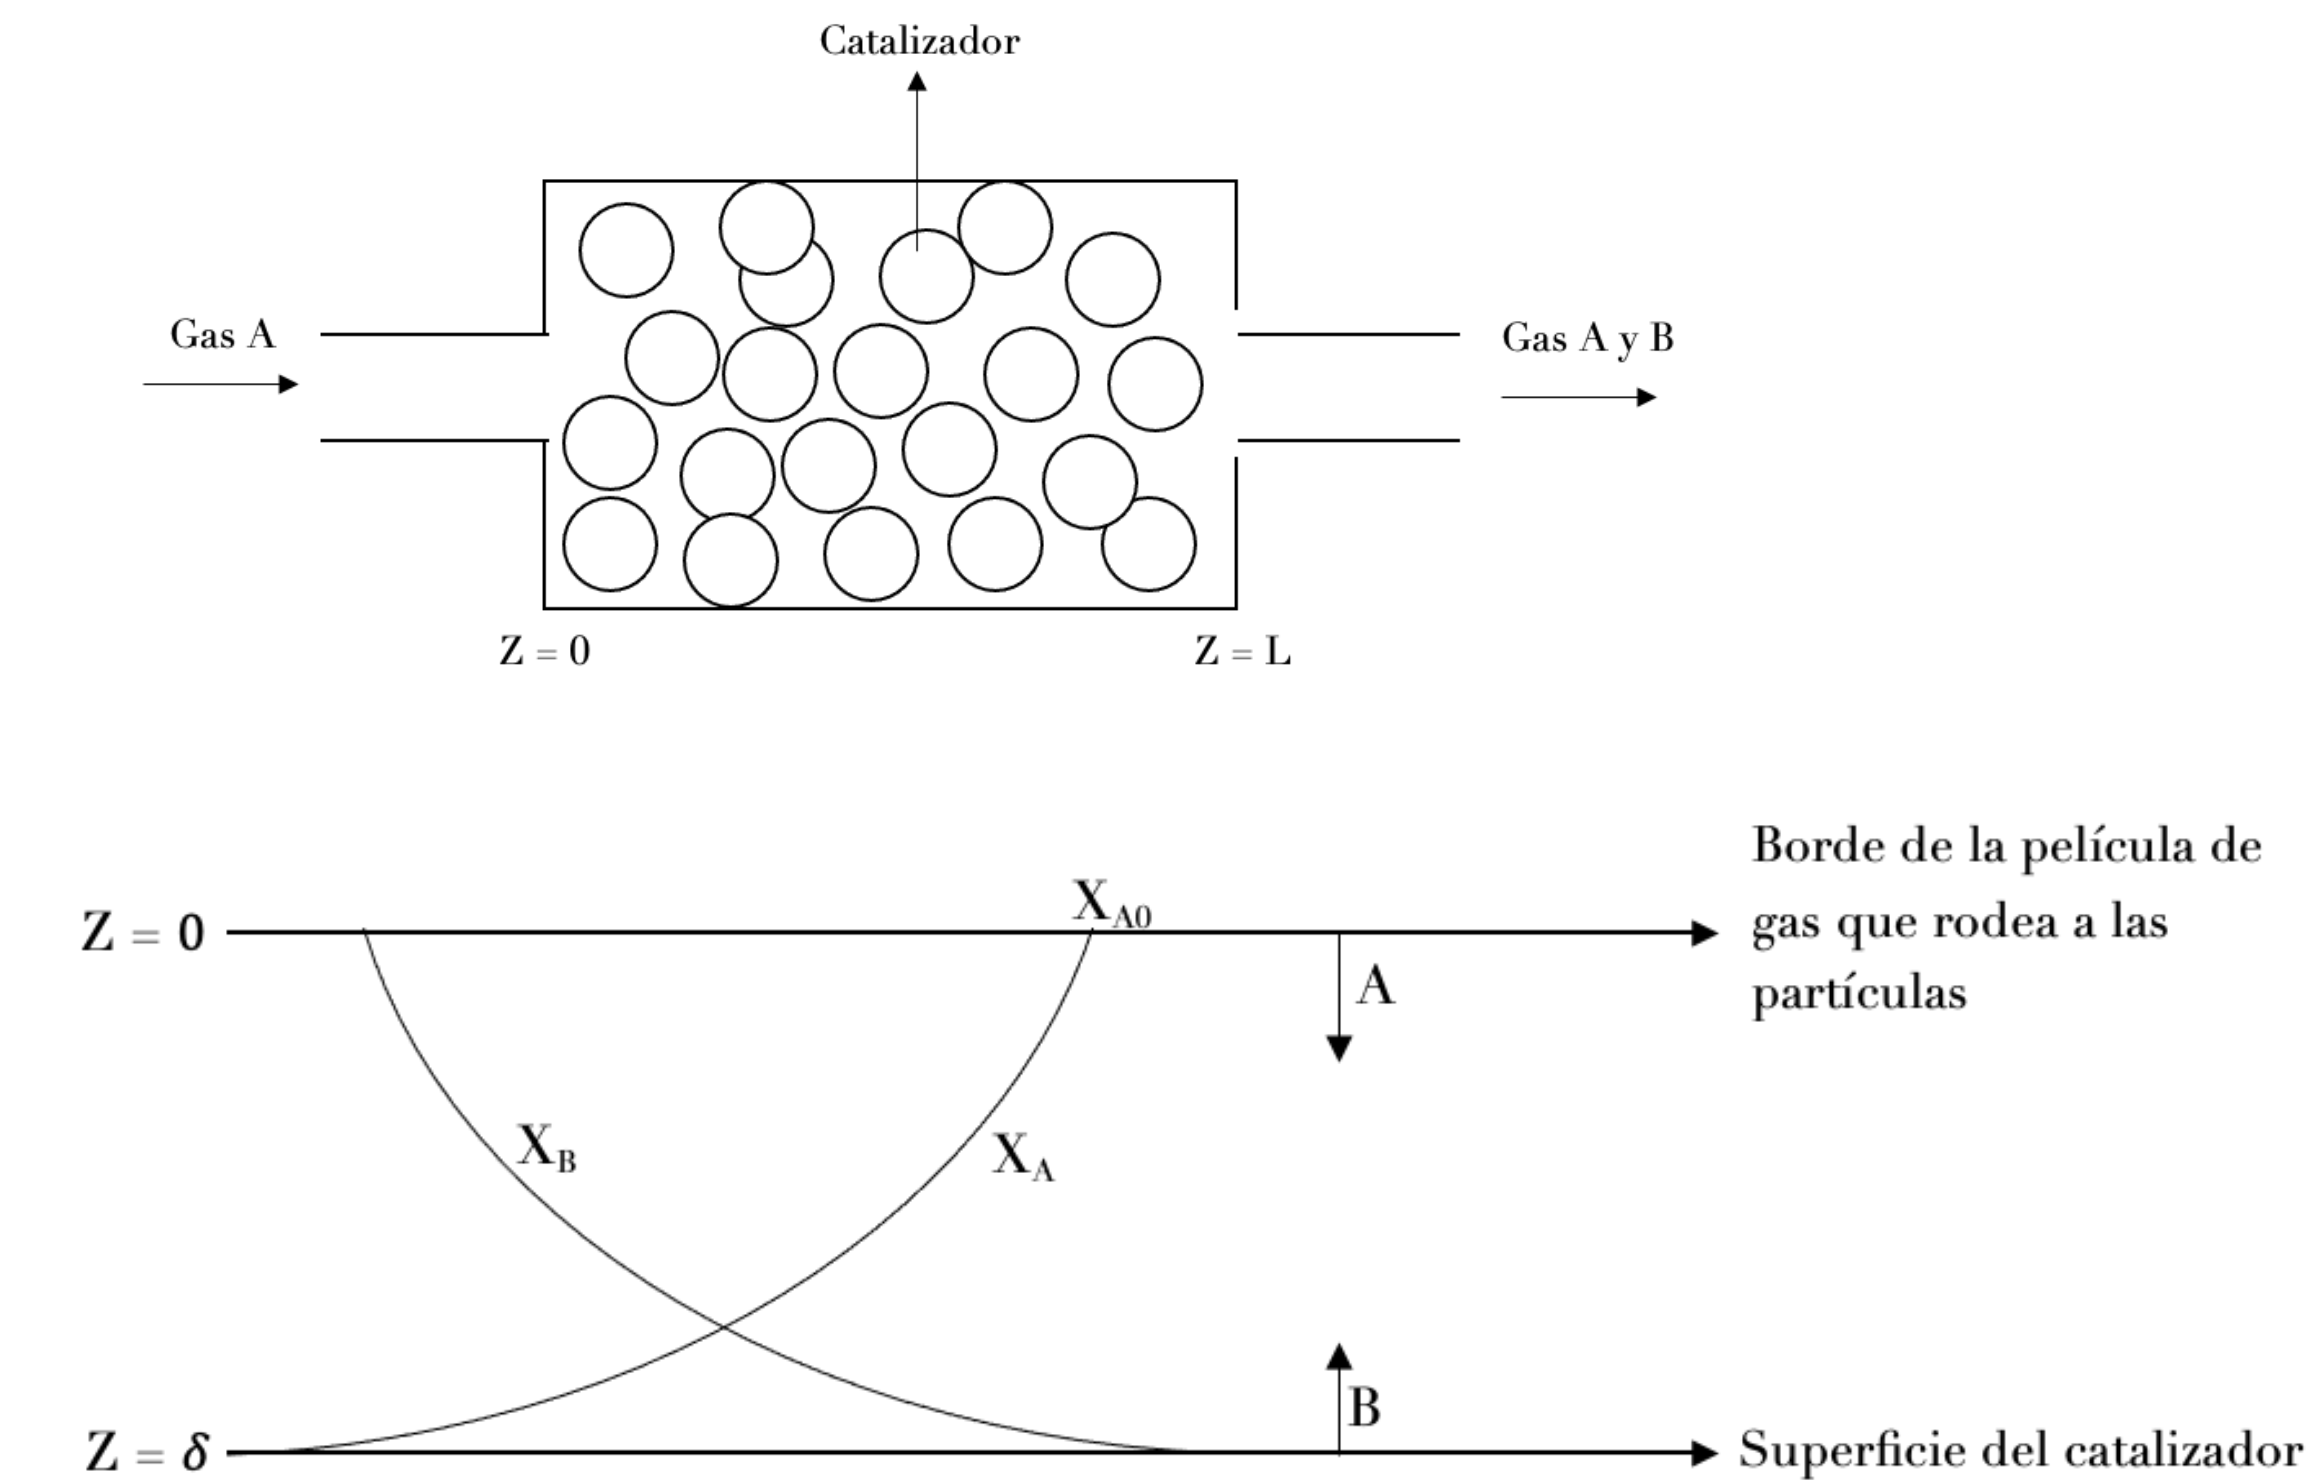
\includegraphics[width=\linewidth]{Capitulo2/Imagenes/Fig_2.12.png}
    \caption{Reactor catalítico en donde $2A\to B$\\Modelo de difusión cerca de la partícula de catalizador}
    \label{fig:fig_2.12}
\end{figure}

2 moles de A se mueven en dirección +z y un mol de B se mueve en dirección -z. Por lo tanto, a régimen permanente:

\begin{equation}
    N_{Bz}=-\frac{1}{2}N_{Az}
    \label{eq_2.71}
\end{equation}

Las ecs \eqref{eq_1.25} y \eqref{eq_1.19} en combinación con la ec \eqref{eq_2.71} son:

\begin{equation}
    N_{Az}=-\frac{c\mathscr{D}_{AB}}{1-\frac{x_A}{2}}\frac{d(x_A)}{dz}
\end{equation}
\begin{equation}
   \text{y} \quad \frac{d(N_A)}{dz}=0
\end{equation}


que resulta en:
\begin{equation}
    \frac{d}{dz}\left(\frac{1}{1-\frac{1}{2}x_A}\frac{dx_A}{dz}\right)=0
    \label{eq_2.74}
\end{equation}




Con las condiciones en la frontera:

\begin{equation}
    x_A |_{z=0} = x_{A0}\quad \text{y} \quad x_A |_{z=\delta} = 0
    \label{eq_2.75}
\end{equation}

A partir de la ec. \eqref{eq_2.74}, se obtiene:

\begin{equation*}
    \frac{1}{1-\frac{x_A}{2}}\frac{dx_A}{dz}=C_1\longrightarrow \int\frac{dx_A}{1-\frac{x_A}{2}}=C_1\int dz +C_2
\end{equation*}

Evaluando $C_1$ y $C_2$ con respecto a las condiciones \eqref{eq_2.75}, se obtiene:

\begin{equation}
    N_{Az}=\frac{2C\mathscr{D}_{AB}}{\delta}\ln\left(\frac{1}{1-\frac{1}{2}x_{A0}}\right)
    \label{eq_2.76}
\end{equation}

La reacción ocurre instantáneamente, por lo que la convección de A en B es un proceso controlado por difusión.

\subsection{Difusión con reacción heterogénea lenta}

En este caso, para el mismo sistema, la reacción no sucede instantáneamente en $z=\delta$, sino que la desaparición de A en la superficie del catalizador es proporcional a la concentración de A en la interfase:

\begin{equation}
    N_{Az}=k_1C_A=k_1Cx_A
\end{equation}

En este caso, la condición de frontera en la superficie del catalizador es:

\begin{equation*}
    x_A|_{z=\delta}=\frac{N_{Az}}{k_1c}
\end{equation*}

El cambio en la condición de frontera, resulta en el siguiente perfil:

\begin{equation}
    \frac{1-\frac{x_A}{2}}{(1-\frac{x_{A0}}{2})^{1-\frac{z}{\delta}}}=\left(1-\frac{N_{Az}}{2k_1c}\right)^{\frac{z}{\delta}}
\end{equation}



\begin{equation}
\begin{split}
     \frac{d}{dz}\ln\left(1-\frac{x_A}{2}\right)-\frac{d}{dz}\left[\left(1-\frac{z}{\delta}\right)\ln\left(1-\frac{x_{A0}}{2}\right)\right]=\frac{d}{dz}\left[\frac{z}{\delta}\ln \left(1-\frac{N_{Az}}{2k_1c}\right)\right]\\-\frac{\frac{1}{2}}{1-\frac{x_A}{2}}\frac{dx_A}{dz}+\frac{1}{\delta}\ln \left(1-\frac{x_{A0}}{2}\right)=\frac{1}{\delta}\ln \left(1-\frac{N_{Az}}{2k_1c}\right)   
\end{split}
\label{eq_2.79}
\end{equation}

Substituyendo la ec \eqref{eq_2.79} en la ec \eqref{eq_2.74}, se obtiene:

\begin{equation*}
    N_{Az}=-\frac{c\mathscr{D}_{AB}}{(1-\frac{x_A}{2})}\left[\left(1-\frac{x_A}{2}\right)\left(\frac{-2}{\delta}\right)\ln \left(\frac{1-\frac{N_{Az}}{k_1c}}{1-\frac{x_{A0}}{2}}\right)\right]
\end{equation*}
Aproximando $\ln (1-\frac{N_{Az}}{2k_1c})\approx -\frac{1}{2}\frac{N_{Az}}{k_1c}$, se obtiene:

\begin{equation*}
   N_{Az}=\frac{2C\mathscr{D}_{AB}}{\delta}\left[-\frac{N_{Az}}{2k_1c}-\ln \left(1-\frac{x_{A0}}{2}\right)\right] 
\end{equation*}
\begin{equation*}
   N_{Az}\left(1+\frac{\mathscr{D}_{AB}}{k_1\delta}\right)=2C\frac{\mathscr{D}_{AB}}{\delta}\ln \left(\frac{1}{1-\frac{1}{2}x_{A0}}\right)  
\end{equation*}
\begin{equation}
   N_{Az}=2c\frac{\mathscr{D}_{AB}}{\delta(1+\frac{\mathscr{D}_{AB}}{k_1\delta})}\ln \left(\frac{1}{1-\frac{1}{2}x_{A0}}\right)  
\end{equation}

El número adimensional $\frac{k_1\delta}{\mathscr{D}_{AB}}=Da$ es el número de Damköler, el cual describe la relación entre reacción y difusión. Si $Da\rightarrow\infty$, se obtiene el caso de reacción dominante y la ecuación toma la forma de la ec. \eqref{eq_2.76}

\section{Difusión con reacción química en medios porosos}

En este caso, se describe la difusión de los reactivos en un medio poroso en términos de una difusividad efectiva ($D_A$). Supóngase que la reacción tiene lugar en la superficie sólida de un catalizador cuya simetría es esférica y posee un radio R, la reacción es $A\rightarrow B$. Esta partícula esférica está sumergida en una corriente de gas con A y B presentes. A se difunde en los poros de la superficie esférica y ahí sucede la reacción. La ec \eqref{eq_1.30} dentro del medio poroso en coordenadas esfericas es:

\begin{equation}
    0=D_A\frac{1}{r^2}\frac{d}{dr}(r^2\frac{d(C_A)}{dr})-R_A
    \label{eq_2.81}
\end{equation}

"a" se define como la superficie catalítica por unidad de volumen (sólido + huecos). Por ello, $R_A=-k_1ac_a$.

Haciendo un cambio de variable, $\frac{C_A}{C_{AR}}=\frac{f(r)}{r}$ en donde $C_{AR}$ es la concentración de A en la superficie esférica, la ec \eqref{eq_2.81} se transforma en:

\begin{equation}
    \frac{d^2f}{dr^2}-\frac{k_1a}{D_A}f=0
    \label{eq_2.82}
\end{equation}

Con condiciones en la frontera:

\begin{equation}
    C_A|_{r=R}=C_{AR} \quad \text{y} \quad C_A|_{r=0}=finito
\end{equation}
o bien:
\begin{equation*}
    f|_{r=R}=R\quad \text{y} \quad
    f|_{r=0}=\text{finito}
\end{equation*}

La solución a la ecuación \eqref{eq_2.82} corresponde a:

\begin{equation}
    f(r)=C_1\cosh[(\frac{k_1a}{D_A})^\frac{1}{2}r]+C_2\sinh[(\frac{k_1a}{D_A})^\frac{1}{2}r]
\end{equation}
\begin{equation*}
    f(0)=C_1=0
\end{equation*}
\begin{equation*}
    f(R)=C_2\sinh[(\frac{k_1a}{D_A})^\frac{1}{2}R]=R\longrightarrow C_2=\frac{R}{sinh[(\frac{k_1a}{D_A})^\frac{1}{2}R]}
\end{equation*}

Por lo tanto:

\begin{equation}
    f(r)=\frac{R\sinh[(\frac{k_1a}{D_A})^\frac{1}{2}r]}{\sinh[(\frac{k_1a}{D_A})^\frac{1}{2}R]}
\end{equation}

Definiendo el modulo de Thiele como $\phi=\sqrt{\frac{k_1a}{D_A}}R$, entonces:
    $f(r)=\frac{R\sinh[\phi(\frac{r}{R})]}{\sinh\phi}$
Luego, 
\begin{equation}
    \frac{C_A}{C_{AR}}=\frac{R}{r}\frac{\sinh[\phi(\frac{r}{R})]}{\sinh\phi}
\end{equation}


Claramente, $\frac{C_A}{C_{AR}}|_{r=0}=\frac{\phi}{\sinh\phi}$ 
\newline
El flujo molar en la superficie es: $W_{AR}=4\pi R^2N_{AR}=-4\pi R^2D_A\frac{d(C_A)}{dr}|_{r=R}$
\begin{equation*}
\begin{split}
        \frac{d(C_A)}{dr}|_{r=R}=\frac{C_{AR}R}{\sinh \phi}\left[\frac{r}{r^2}\cosh\left[\frac{\phi r}{R}\right]\left(\frac{\phi}{R}\right)-\frac{1}{r^2}\sinh \left[\frac{\phi r}{R}\right]\right]\\
=\frac{C_{AR}R}{\sinh (\phi)}\left[\frac{\phi}{R^2}\cosh \phi-\frac{\sinh \phi}{R^2}\right]=\frac{C_{AR}}{R}[\phi \coth \phi-1]
\end{split}
\end{equation*}

Por lo tanto:

\begin{equation}
    W_{AR}=4\pi RC_{AR}D_A[1-\phi \coth (\phi)]
    \label{eq_2.87}
\end{equation}

Definiendo al factor de efectividad $\eta$:

\begin{equation}
    \eta=\frac{N_{AR}}{N_{AR0}}
    \label{eq_2.88}
\end{equation}
En donde $N_{AR0}$ es el flujo molar sin efectos difusionales, es decir:

\begin{equation}
    N_{AR0}=\frac{4\pi R^3}{3}a(-k_1C_{AR})
    \label{eq_2.89}
\end{equation}

Sustituyendo las ecs \eqref{eq_2.87} y \eqref{eq_2.89} en la ec \eqref{eq_2.88} resulta en: 

\begin{equation}
    \eta_A=\frac{3}{\phi^2}[\phi \coth (\phi)-1]
    \label{eq_2.90}
\end{equation}

Físicamente, $\eta_A$ es el factor tal que $\eta_AW_{AR0}$ representa la resistencia difusional del proceso. Para partículas no esféricas, el radio $R_{n e}$ se define como:

\begin{equation}
    R_{ne}=3\left(\frac{V_p}{S_p}\right)
\end{equation}

De tal forma que para partículas esféricas: $\frac{V_p}{S_p}=\frac{\frac{4\pi R^3}{3}}{4\pi R^2}=\frac{R}{3}$

En este caso, el valor de conversión absoluto en la reacción corresponde a:
\begin{equation*}
    |W_{AR}|=V_pak_1C_{AR}\eta_A
\end{equation*}
y donde ahora:
\begin{equation}
    \eta_A=\frac{1}{3\Lambda^2}(3\Lambda \coth 3\Lambda-1)
\end{equation} 
y
\begin{equation}
    \Lambda=(\frac{k_1a}{D_A})^{\frac{1}{2}}(\frac{V_p}{S_p})
\end{equation}
Es el modulo de Thiele generalizado. La variación de $\eta_A$ en función de $\Lambda$ se grafica en la fig \eqref{fig:fig_2.13} para diferentes geometrías

\begin{figure}[H]
    \centering
    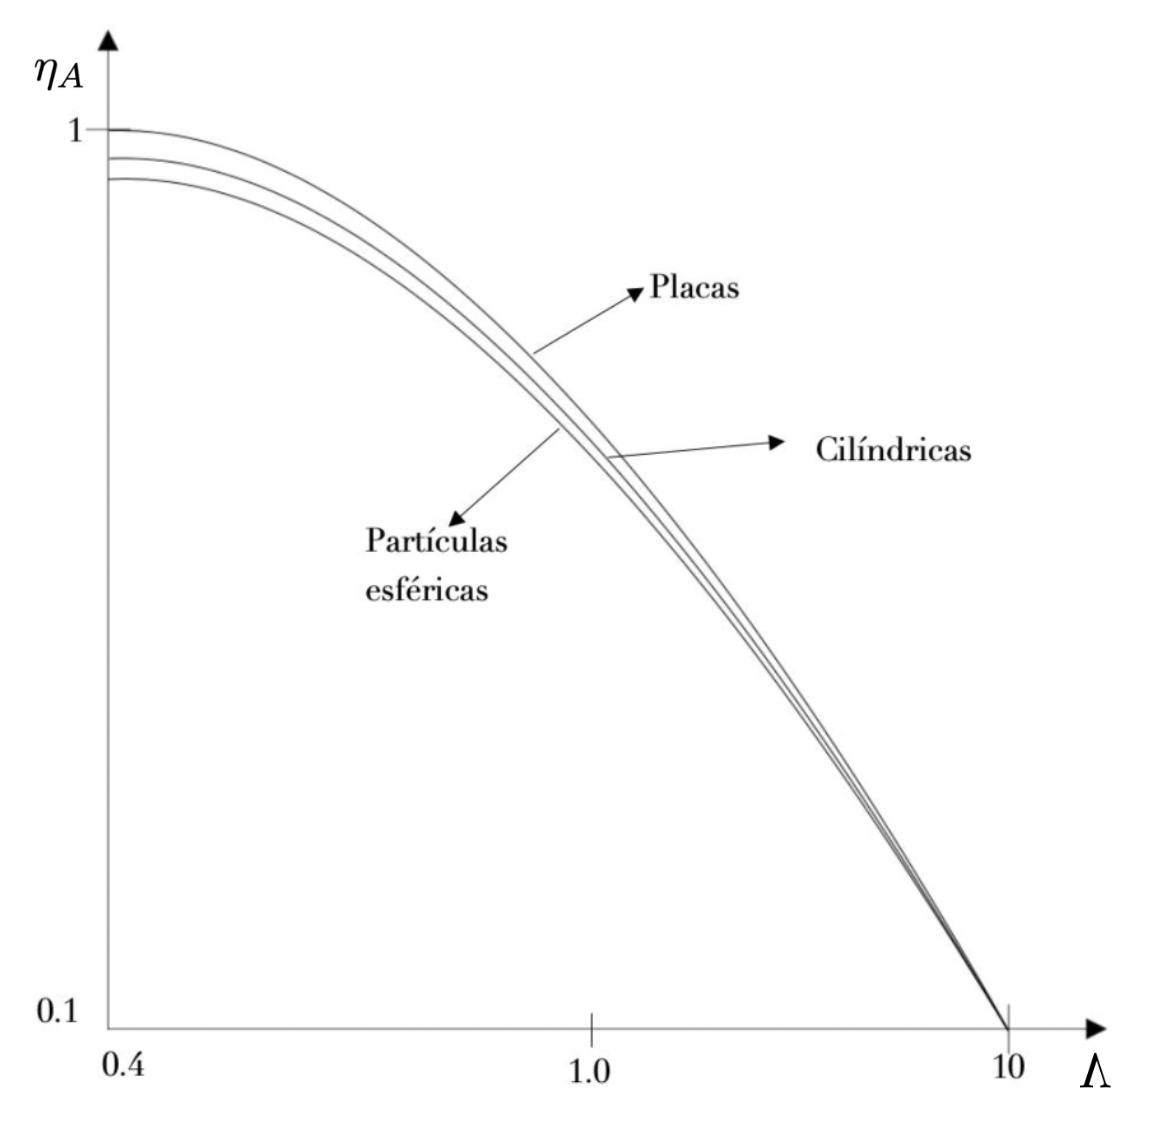
\includegraphics[width=0.7\linewidth]{Capitulo2/Imagenes/Fig_2.13.png}
    \caption{Factores de efectividad en catalizadores porosos de varias fromas}
    \label{fig:fig_2.13}
\end{figure}
\newpage
\section*{Apéndice A}
\begingroup
\renewcommand{\thefigure}{A.\arabic{figure}}
\setcounter{figure}{0}
\renewcommand{\theequation}{A.\arabic{equation}} 
\setcounter{equation}{0}
Difusión debido a una fuente puntual en una corriente de fluído.
Un fluido B fluye a una velocidad constante $v_0$. en algún punto, la especie A se inyecta a un flujo $W_A$ (gmol/s) que es suficientemente pequeño. A se difunde axial y radialmente.

Como este es un problema de convección-difusión, en coordenadas cilíndricas (vea la ec. \eqref{eq_B} en el apéndice B), en la dirección z, se tiene:

\begin{equation}
    \frac{\partial C_A}{\partial t}+v_z\frac{\partial C_A}{\partial z}=\mathscr{D}_{AB}\left[\frac{1}{r}\frac{\partial }{\partial r}\left(r\frac{\partial C_A}{\partial r}\right)+\frac{\partial ^2C_A}{\partial z^2}\right]
\end{equation}
en donde $dt=\frac{dz}{v_0}$.

Ahora, se realiza un cambio de variable $C_A(r,z)=C_A(s,z)$, en la cual $s^2=r^2+z^2$ (ver fig. \eqref{fig:Fig_A.1.})
\begin{figure}[H]
    \centering
    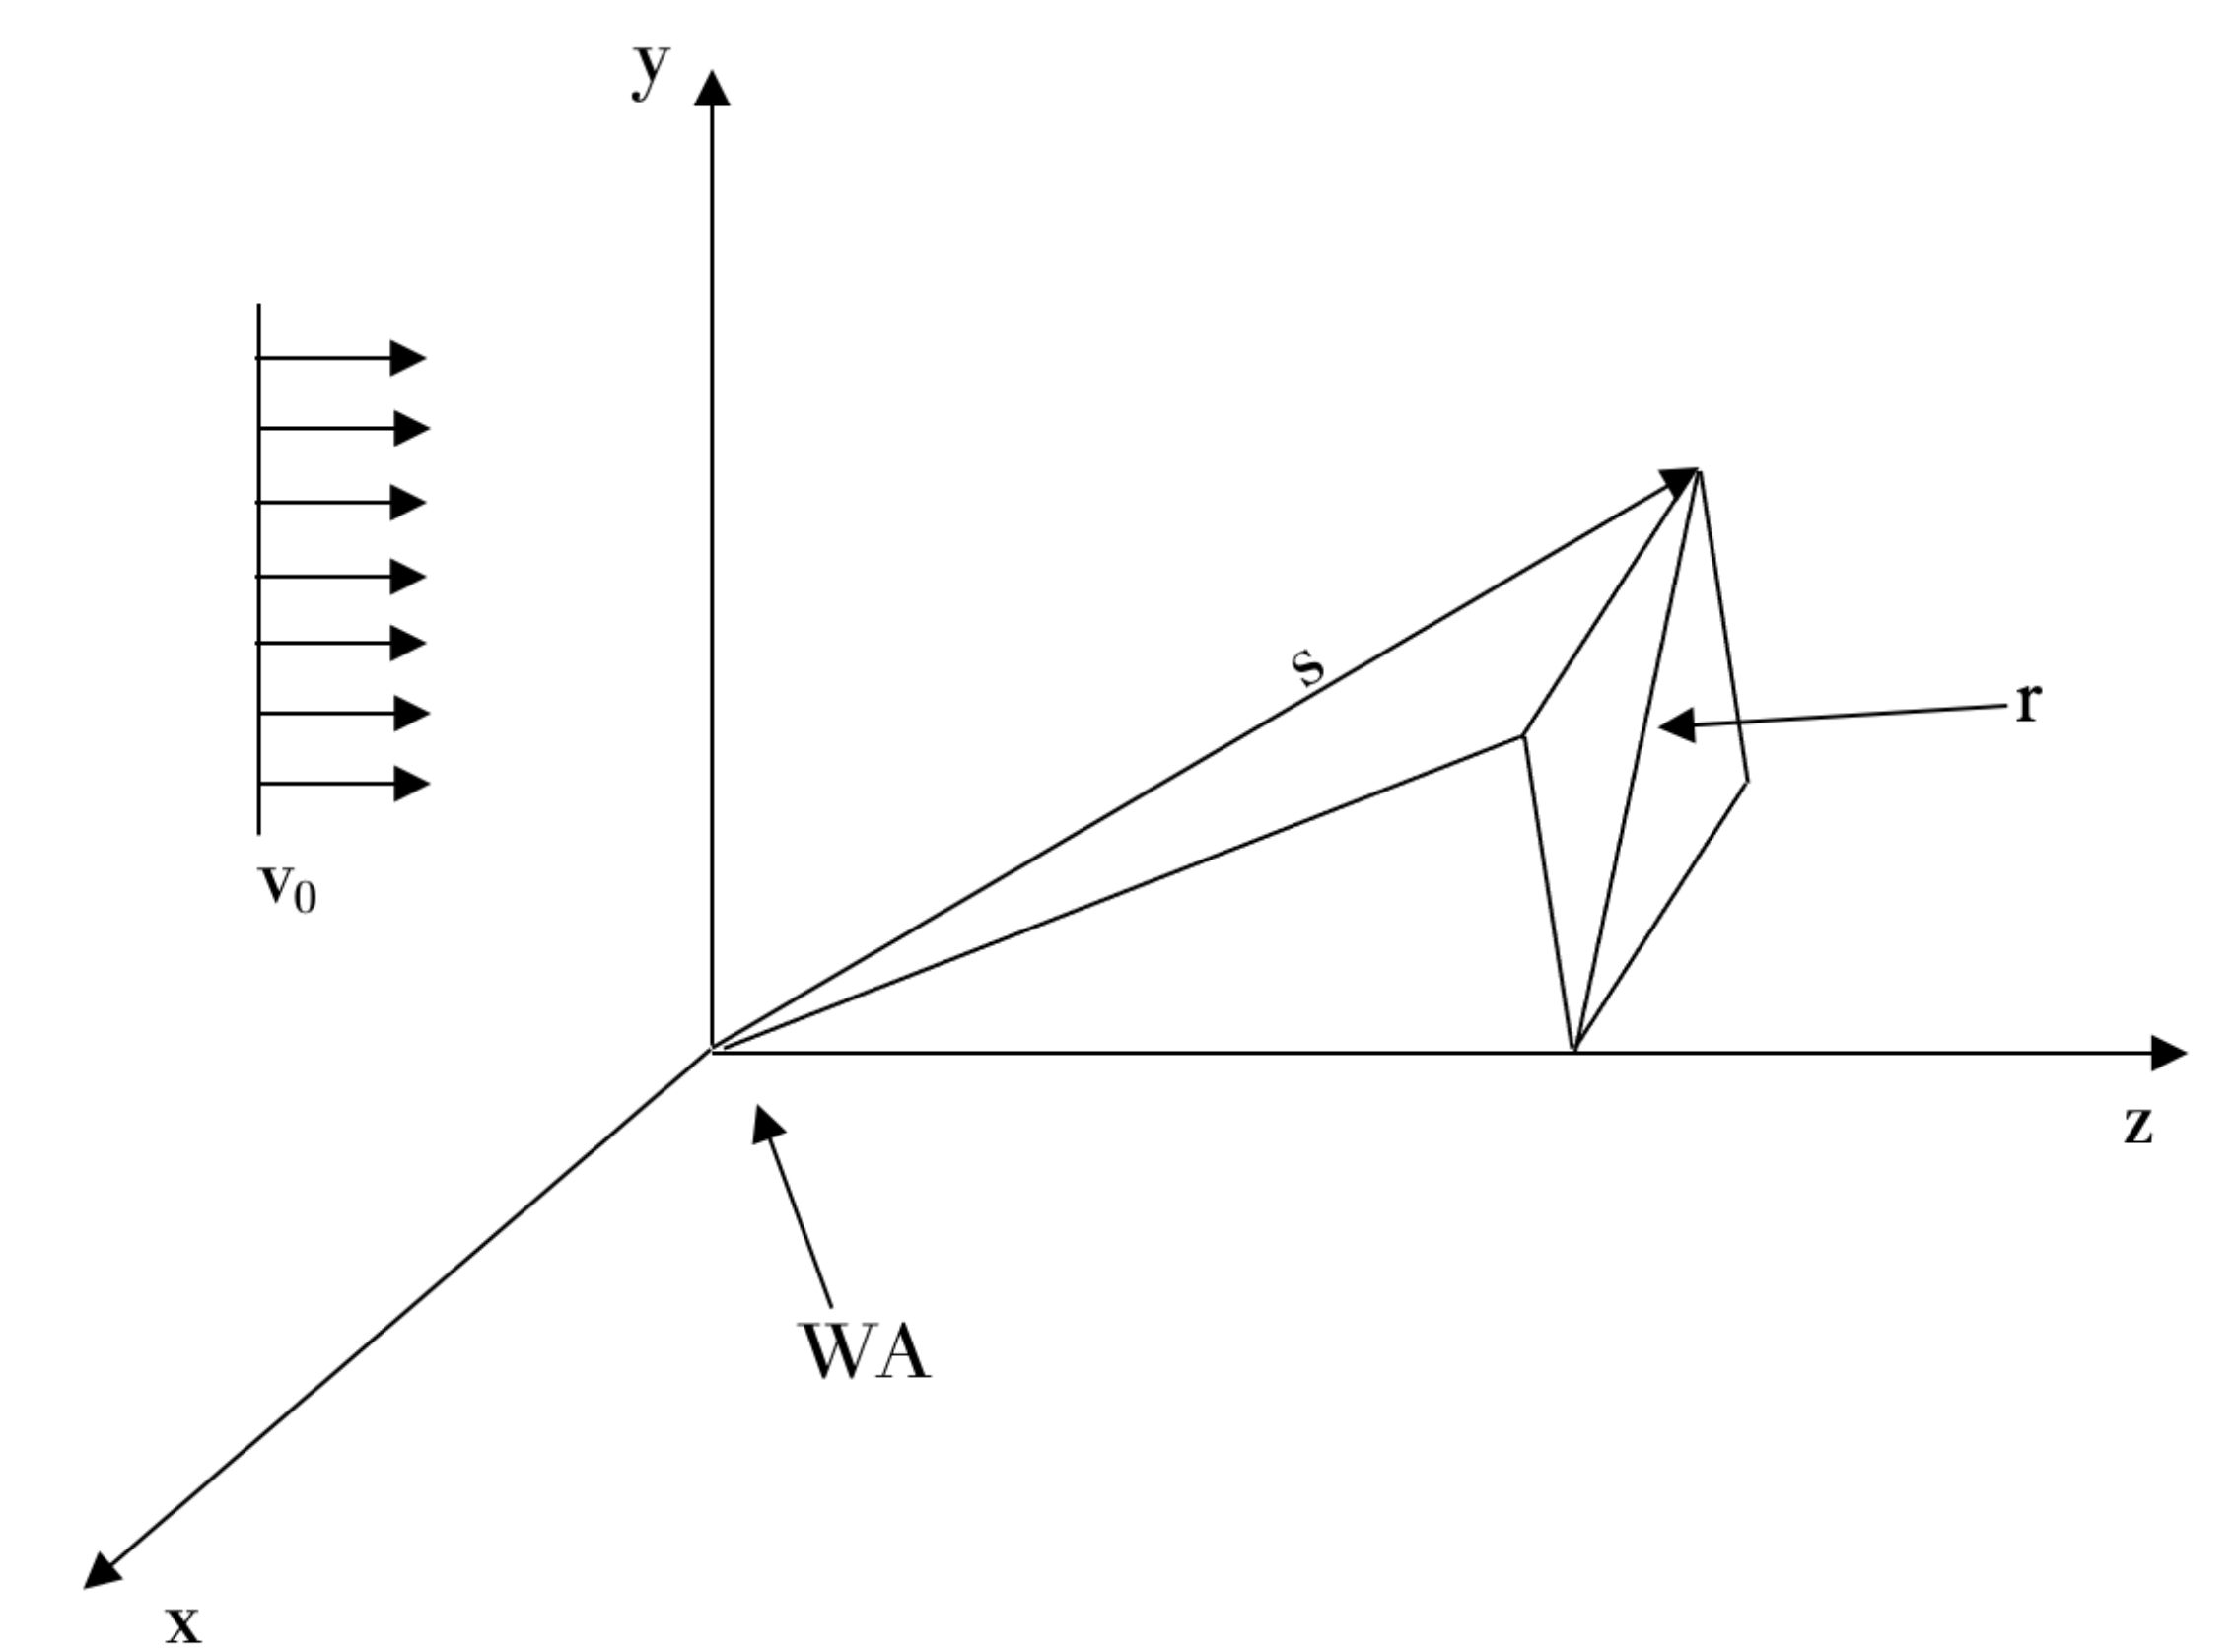
\includegraphics[width=0.5\linewidth]{Capitulo2/Imagenes/Fig_A.1.png}
    \caption{Difusión de A desde una fuente puntual en una corriente de B que va a una velocidad $v_0$ constante}
    \label{fig:Fig_A.1.}
\end{figure}

El diferencial $dC_A$ por regla de la cadena, corresponde a:

\begin{equation*}
    dC_A=(\frac{\partial C_A}{\partial s})_zds+(\frac{\partial C_A}{\partial z})_sdz
\end{equation*}
Luego:
\begin{equation*}
    (\frac{\partial C_A}{\partial z})_r=(\frac{\partial C_A}{\partial s})_z\frac{ds}{dz}+(\frac{\partial C_A}{\partial z})_s
\end{equation*}
Recordando que $s^2=r^2+z^2$, por lo tanto, $\frac{\partial s}{\partial z}=\frac{z}{s}$
\begin{equation*}
    (\frac{\partial C_A}{\partial z})_r=(\frac{\partial C_A}{\partial s})_z\frac{z}{s}+(\frac{\partial C_A}{\partial z})_s
\end{equation*}

\begin{equation*}
    (\frac{\partial^2C_A}{\partial z^2})_r=\frac{\partial}{\partial z}((\frac{dC_A}{dz})_r)
\end{equation*}
\begin{equation*}
    (\frac{\partial^2C_A}{\partial z^2})_r=[\frac{\partial}{\partial s}((\frac{\partial C_A}{\partial s})_r)\frac{\partial s}{\partial z}+\frac{\partial }{\partial z}((\frac{\partial C_A}{\partial s})_r)]_s
\end{equation*}
\begin{equation*}
    (\frac{\partial^2C_A}{\partial z^2})_r=\frac{\partial}{\partial s}[(\frac{\partial C_A}{\partial s})_z\frac{z}{s}+(\frac{\partial C_A}{\partial z})_s]\frac{z}{s}+\frac{\partial }{\partial z}[(\frac{\partial C_A}{\partial s})_z\frac{z}{s}+(\frac{\partial C_A}{\partial z})_s]
\end{equation*}
\begin{equation*}
    (\frac{\partial^2C_A}{\partial z^2})_r=\frac{z}{s}[(\frac{\partial^2 C_A}{\partial s^2})_z\frac{z}{s}-(\frac{\partial C_A}{\partial s})_z\frac{z}{s^2}+\frac{\partial^2C_A}{\partial s \partial z}]
\end{equation*}
\begin{equation*}
    +[(\frac{\partial^2C_A}{\partial z \partial s})\frac{z}{s}+(\frac{\partial C_A}{\partial s})_s\frac{1}{s}+(\frac{\partial^2C_A}{\partial z^2})_s]
\end{equation*}
Se calculan ahora, las derivadas radiales:

\begin{equation*}
    (\frac{\partial C_A}{\partial r})_z=(\frac{\partial C_A}{\partial s})_z(\frac{\partial s}{\partial r})_z=(\frac{\partial C_A}{\partial s})_z(\frac{r}{s})=(\frac{\partial C_A}{\partial s})_z(\frac{(s^2-z^2)^\frac{1}{2}}{s})
\end{equation*}
\begin{equation*}
     r(\frac{\partial C_A}{\partial r})_z=(\frac{\partial C_A}{\partial s})_z(\frac{s^2-z^2}{s})
\end{equation*}
\begin{equation*}
    \frac{1}{r}\frac{\partial}{\partial r}(r(\frac{\partial C_A}{\partial r})_z)=\frac{1}{s}\frac{\partial}{\partial s}[(\frac{s^2-z^2}{s})(\frac{\partial C_A}{\partial s})_z]
\end{equation*}
\begin{equation*}
    =\frac{1}{s}[(\frac{s^2-z^2}{s})(\frac{\partial C_A}{\partial s})_z]+(\frac{s^2-z^2}{s})(\frac{\partial^2C_A}{\partial s^2})_z
\end{equation*}

Sumando, se obtiene:
\begin{equation*}
    \frac{\partial^2C_A}{\partial z^2}+2\frac{z}{s}\frac{\partial^2C_A}{\partial s \partial z}+\frac{\partial^2C_A}{\partial s^2}+\frac{z}{s}(\frac{\partial C_A}{\partial s})
\end{equation*}
O de manera equivalente:
\begin{equation*}
    \frac{\partial^2C_A}{\partial z^2}+2\frac{z}{s}\frac{\partial^2C_A}{\partial s \partial z}+\frac{1}{s^2}\frac{\partial}{\partial s}(s^2\frac{\partial C_A}{\partial s})=f(s,r,z)
\end{equation*}
Al insertar en la ecuación (A.1), se obtiene:
\begin{equation*}
    v_0(\frac{z}{s}\frac{\partial C_A}{\partial s}+\frac{\partial C_A}{\partial z})=\mathscr{D}_{AB}f(s,r,z)
\end{equation*}
Cuya solución es:
\begin{equation}
    C_A=[\frac{W_A}{4\pi \mathscr{D}_{AB}s}]e^{\frac{-v_0(s-z)}{2\mathscr{D}_{AB}}}
\end{equation}
Que satisface las condiciones de frontera:
\begin{equation*}
    1) C_A|_{z \rightarrow \infty}=0 
\end{equation*}
La concentración de A lejos de la fuente es 0
\begin{equation*}
    2) -\frac{\partial C_A}{\partial s}|_{s \rightarrow0}=\frac{W_A}{4\pi \mathscr{D}_{AB}s^2}
\end{equation*}
Este corresponde al sitio de la fuente
\begin{equation*}
    \frac{\partial C_A}{\partial s}=\frac{\partial}{\partial s}[\frac{a}{s}e^{b(s-z)}]=a[\frac{b}{s}e^{b(s-z)}-\frac{1}{s^2}e^{b(s-z)}]=ae^{b(s-z)}[\frac{b}{s}-\frac{1}{s^2}]
\end{equation*}
En donde $a=\frac{W_A}{4\pi \mathscr{D}_{AB}}$, entonces. Si $s\rightarrow 0$, recordando que $s^2=z^2+r^2$, tanto r como z deben tender a 0, por lo tanto:
\begin{equation*}
    \frac{\partial C_A}{\partial s}|_{s\rightarrow 0}=\quad\lim_{s\rightarrow0}ae^{b(s-z)}[\frac{b}{s}-\frac{1}{s^2}]
\end{equation*}
Se toma la siguiente consideración, en el límite $\frac{1}{s^2}>>\frac{b}{s}$ y $e^{b(s-z)=1}$. Por lo tanto:
\begin{equation*}
     \frac{\partial C_A}{\partial s}|_{s\rightarrow 0}=a(-\frac{1}{s^2})
\end{equation*}
y finalmente:
\begin{equation*}
   -\frac{\partial C_A}{\partial s}|_{s\rightarrow 0}=\frac{W_A}{4\pi \mathscr{D}_{AB}s^2} 
\end{equation*}
 \begin{equation*}
     3) \frac{\partial C_A}{\partial r}|_{r\rightarrow0}=0
 \end{equation*}
 Lo cual implica que la concentración máxima está en el eje z
 \begin{equation*}
    \frac{\partial C_A}{\partial r}=\frac{\partial C_A}{\partial s}\frac{\partial s}{\partial r}=\frac{r}{s}\frac{\partial C_A}{\partial s}=\frac{r}{s}(ae^{b(s-z)}[\frac{b}{s}-\frac{1}{s^2}])
 \end{equation*}
 si $r\rightarrow0$, $s\rightarrow z$ y el valor de la derivada es igual a 0, lo que nos dice que el máximo de la función $C_A$ está en el eje z.
 A partir de datos de $v_0$ y $W_A$ dados, se puede plantear un modelo de regresión lineal para la determinación de $\mathscr{D}_{AB}$.
 \begin{equation*}
     ln(C_As)=ln(\frac{W_A}{4\pi \mathscr{D}_{AB}})-v_0\frac{(s-z)}{2\mathscr{D}_{AB}}
 \end{equation*}
 En donde $s-z$ es la variable independiente y $C_{AS}$ la variable dependiente.

\begin{figure}[H]
    \centering
    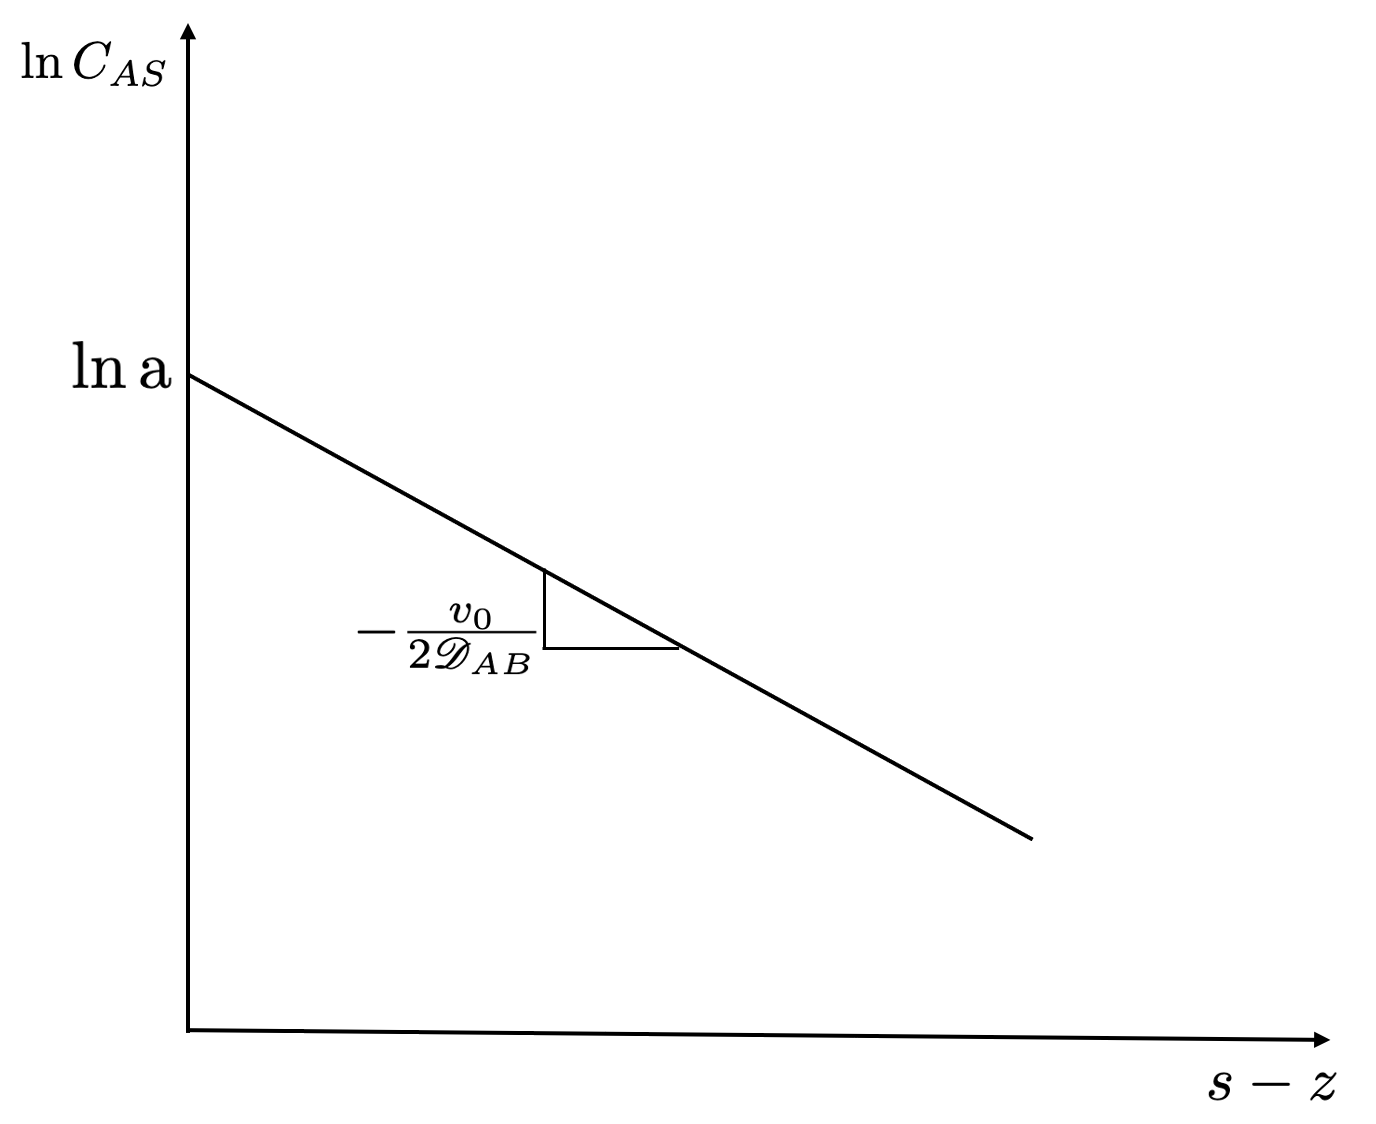
\includegraphics[width=0.5\linewidth]{Capitulo2/Fig_A2.png}
\end{figure}
\endgroup
 

\newpage
\section*{Tarea 2}

\textbf{1. Absorción de cloro en una película descendente}\textit{(Problema. 18A.4, Bird et al.)}
\flushleft
\begin{minipage}{0.3\textwidth} % Tamaño del bloque de la imagen
    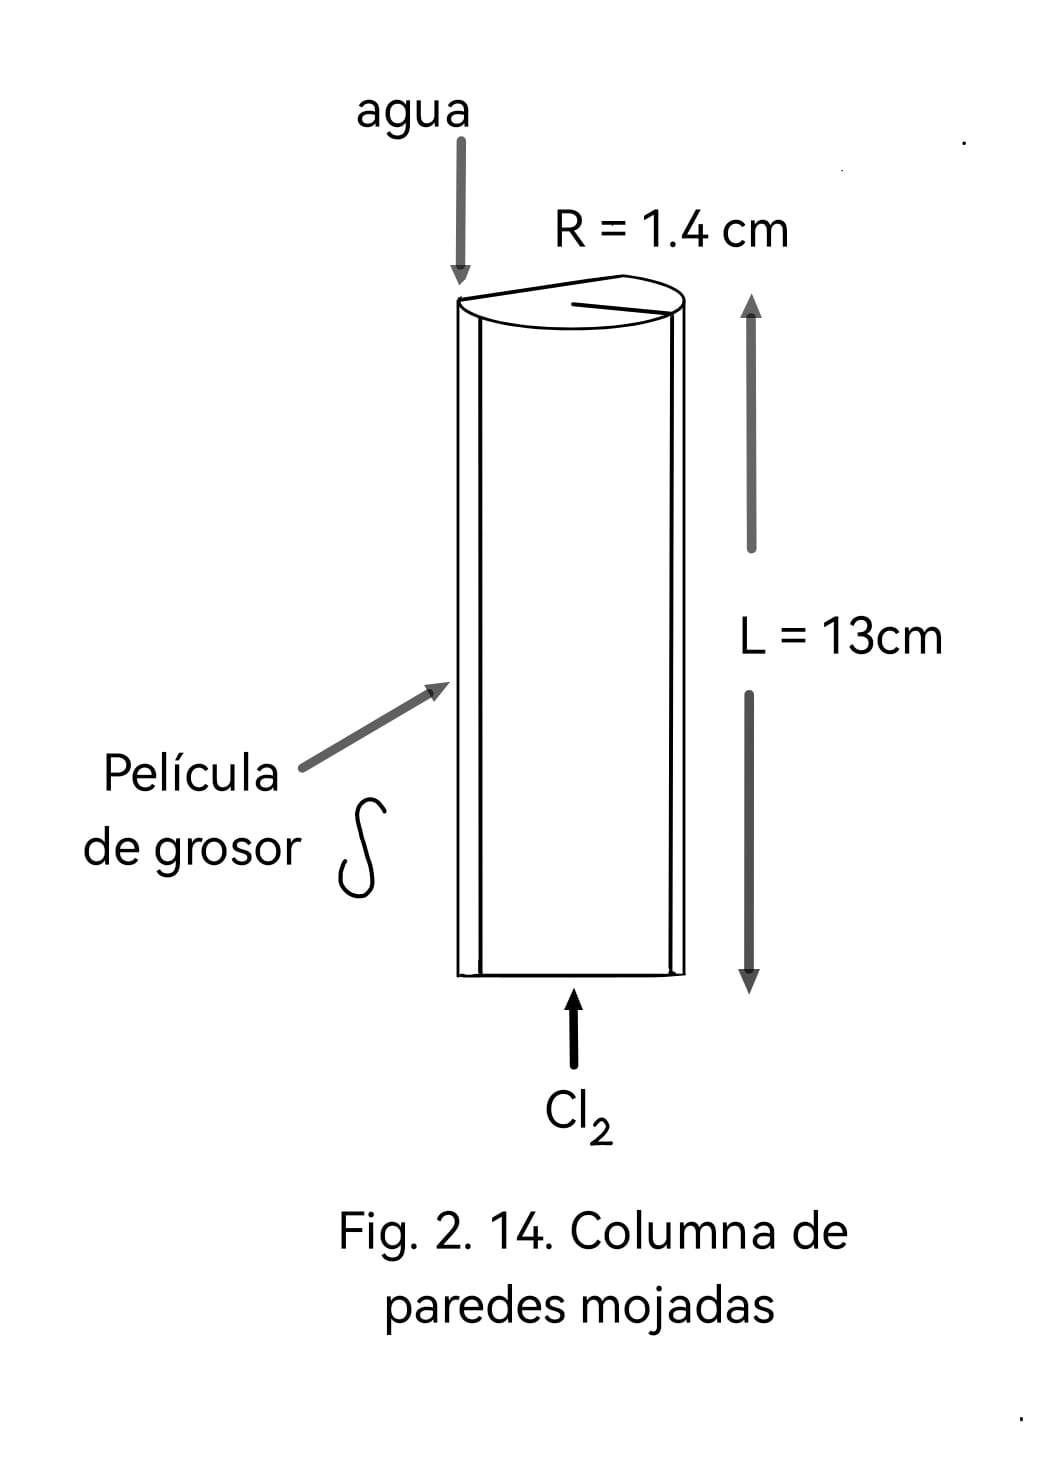
\includegraphics[width=\linewidth]{./Capitulo2/Imagenes/imagen-1.jpg} % Imagen ajustada al bloque
\end{minipage}
\hfill % Espaciado entre imagen y texto
\begin{minipage}{0.65\textwidth} % Tamaño del bloque del texto
Cloro gaseoso se absorbe en agua de la columna de la Fig. 2.14. La velocidad del agua es 17.7 cm/s. La difusividad en la fase líquida del sistema Cl$_2$-H$_2$O es de $1.26 \times 10^{-5}$ cm$^2$/s y la concentración de saturación es de 0.823 g Cl$_2$/100 g H$_2$O. ¿Cuál es la velocidad de absorción en mol/hr?
\vspace{0.5cm} % Espacio antes de la respuesta 
\flushleft
\textbf{Respuesta:} \quad 0.273 \text{ gmol/hr}
\end{minipage}
\vspace{0.5cm} 

\textbf{2.Método para separar helio del gas natural} \textit{(Problema. 18.B.8, Bird et al.)}
\flushleft
\vspace{0.4cm}
\begin{minipage}{0.4\textwidth} % Tamaño del bloque de la imagen
    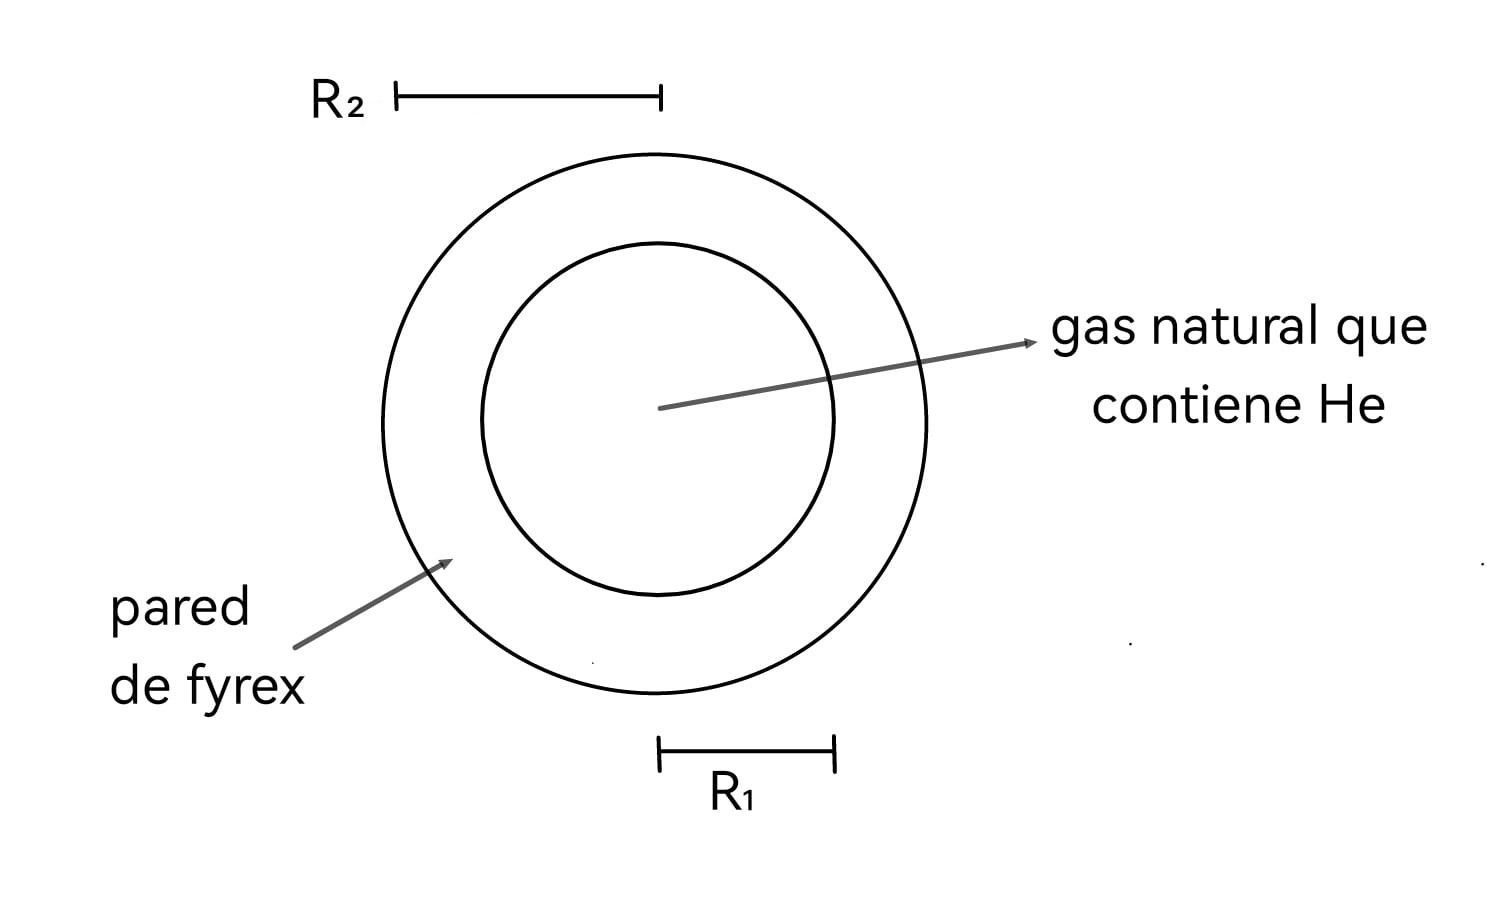
\includegraphics[width=\linewidth]{./Capitulo2/Imagenes/imagen-2.jpg} % Imagen ajustada al bloque
\end{minipage}
\hfill % Espaciado entre imagen y texto
\begin{minipage}{0.55\textwidth} % Tamaño del bloque del texto
La pared de vidrio Pyrex es permeable solamente al He.Suponga que el He está contenido en el recipiente. Obtenga una expresión de la difusión del He a través de la pared, las concentraciones interfaciales del He en las paredes y las dimensiones del tubo.
\vspace{0.5cm} % Espacio antes de la respuesta 
\flushleft
\textbf{Respuesta:
\[
W_{He} = \frac{2\pi L \mathscr{D}_{He} (C_{He_{1}} - C_{He_{2}})}{\ln (R_2/R_1)}
\]}
\end{minipage}
\vspace{0.5cm}

\flushleft
\textbf{3. Velocidad de lixiviación} \textit{(Problema. 18.B.9, Bird et al.)}
\flushleft
\begin{minipage}{0.4\textwidth} % Tamaño del bloque de la imagen
    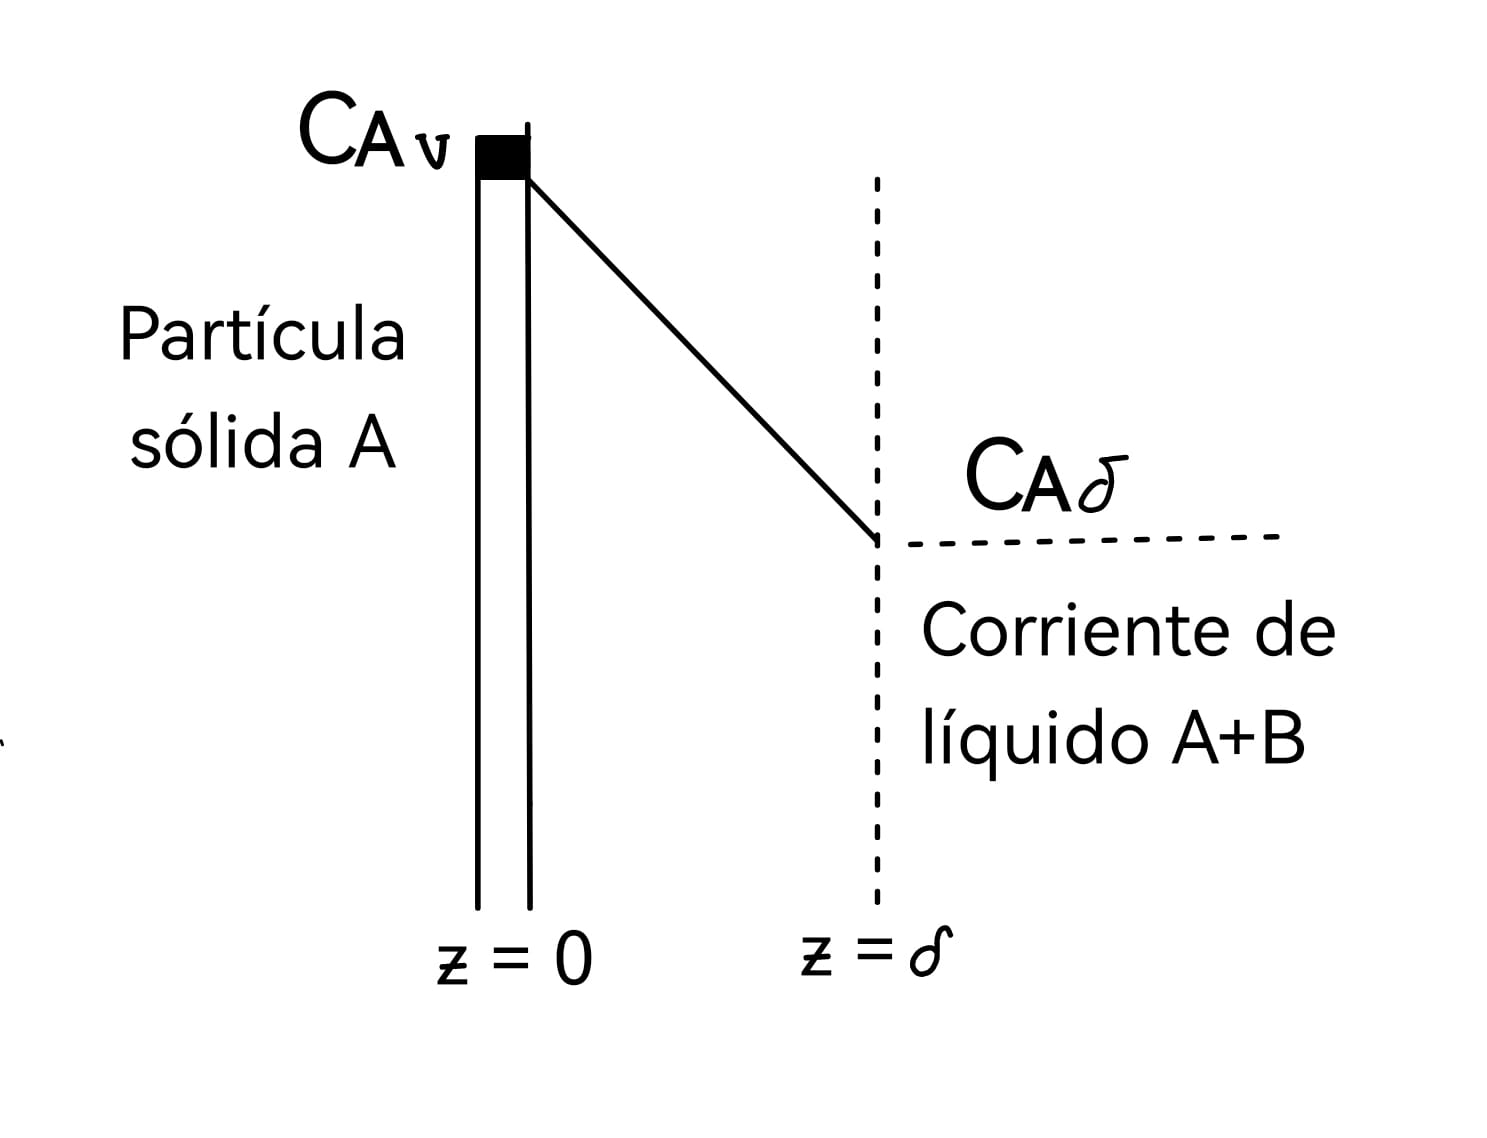
\includegraphics[width=\linewidth]{./Capitulo2/Imagenes/imagen-3.jpg} % Imagen ajustada al bloque
\end{minipage}
\hfill % Espaciado entre imagen y texto
\begin{minipage}{0.5\textwidth} % Tamaño del bloque del texto
La solubilidad de A en B en C$_Au$, y su concentración en B en C$_{A\delta}$. En este proceso, A difunde en B a través de una película de grosor $\delta$. Muestra que al perfil de concentraciones en lineal y que la velocidad de lixiviación es: \[N_{Au}= \frac{\mathscr{D}_{AB}}{C_{Au}-C_{A\delta}}\]
\end{minipage}
\vspace{0.1cm} % Espacio antes de la respuesta 
\flushleft

\textbf{4. Determinación de la difusividad del sistema éter-aire.}\textit{(Problema. 18.A.6 Birt et al)}
\vspace{0.2cm}
\flushleft
Datos de la evaporación del etil-éter con densidad del líquido de $0.7132 \text{ g/cm}^3$. El tubo tiene $6.16 \text{ mm}$ de diámetro y presión total de $747 \text{ mmHg}$  a $22^\circ C$. El peso molecular del éter $74$  y la presión de vapor a $22^\circ C$ en $498 \text{ mmHg}$. (Véase Fig. 2.1)
\vspace{0.2cm}
\flushleft
a)- Suponer un promedio de las longitudes de $Z_2 - Z_1$ para encontrar $\mathscr{D}_{AB}$ a $747 \text{ mmHg}$ y $22^\circ C$ a partir de los datos de evaporación.
\flushleft
b)- Utilizar la ecuación $(1.53)$ para convertir los resultantes a $0^\circ C$ y $760\text{ mmHg}$ .

\begin{table}[h]
    \centering
    \begin{tabular}{cc} % Ambas columnas centradas
        \toprule
        Nivel del éter (mm) & Tiempo (s) para alcanzar el nivel del éter \\
        \midrule
        9-11  & 590  \\
        14-16 & 845  \\
        19-21 & 1185 \\
        24-26 & 1480 \\
        34-34 & 2055 \\
        41-46 & 2655 \\
        \bottomrule
    \end{tabular}
\end{table}

\textbf{Respuesta:} \[
\mathscr{D}_{AB} = 0.0786 \quad \text{cm}^2/\text{s} \quad \text{a} \quad 0^\circ C \quad \text{y} \quad 760 \text{ mmHg}
\]
\newpage
\section*{Tarea 3}
\vspace{0.3cm} % Espacio antes de la respuesta 
\flushleft
\textbf{1. Mediciones de difusividad por el Método de fuente puntual.}\textit{(Problema. 18.A.5 Birt et al.)}
\vspace{0.1cm} % Espacio antes de la respuesta 
\flushleft
Una corriente de líquido B se dirige en dirección vertical, y la composición del gas se mide en varias posiciones. Calcular el gasto molar $W_A$ (g-mol/s) requerido para producir $X_A = 0.01$ en el punto 1 cm abajo de la fuente a 1 atm y $800^\circ$C, si $V_0 = 50$ cm/s y $\mathscr{D}_{AB} = 5$ cm\textsuperscript{2}/s. 
\vspace{0.1cm} % Espacio antes de la respuesta 
\flushleft
Utilizar los resultados del \textbf{Apéndice A}.\\
\flushleft
\textbf{2. Experimentos para medir la difusividad de gases en un aparato de dos recipientes} \textit{(Prob. 18.B.6. Bird et al.)} 
\flushleft
\begin{minipage}{0.5\textwidth} % Tamaño del bloque de la imagen
    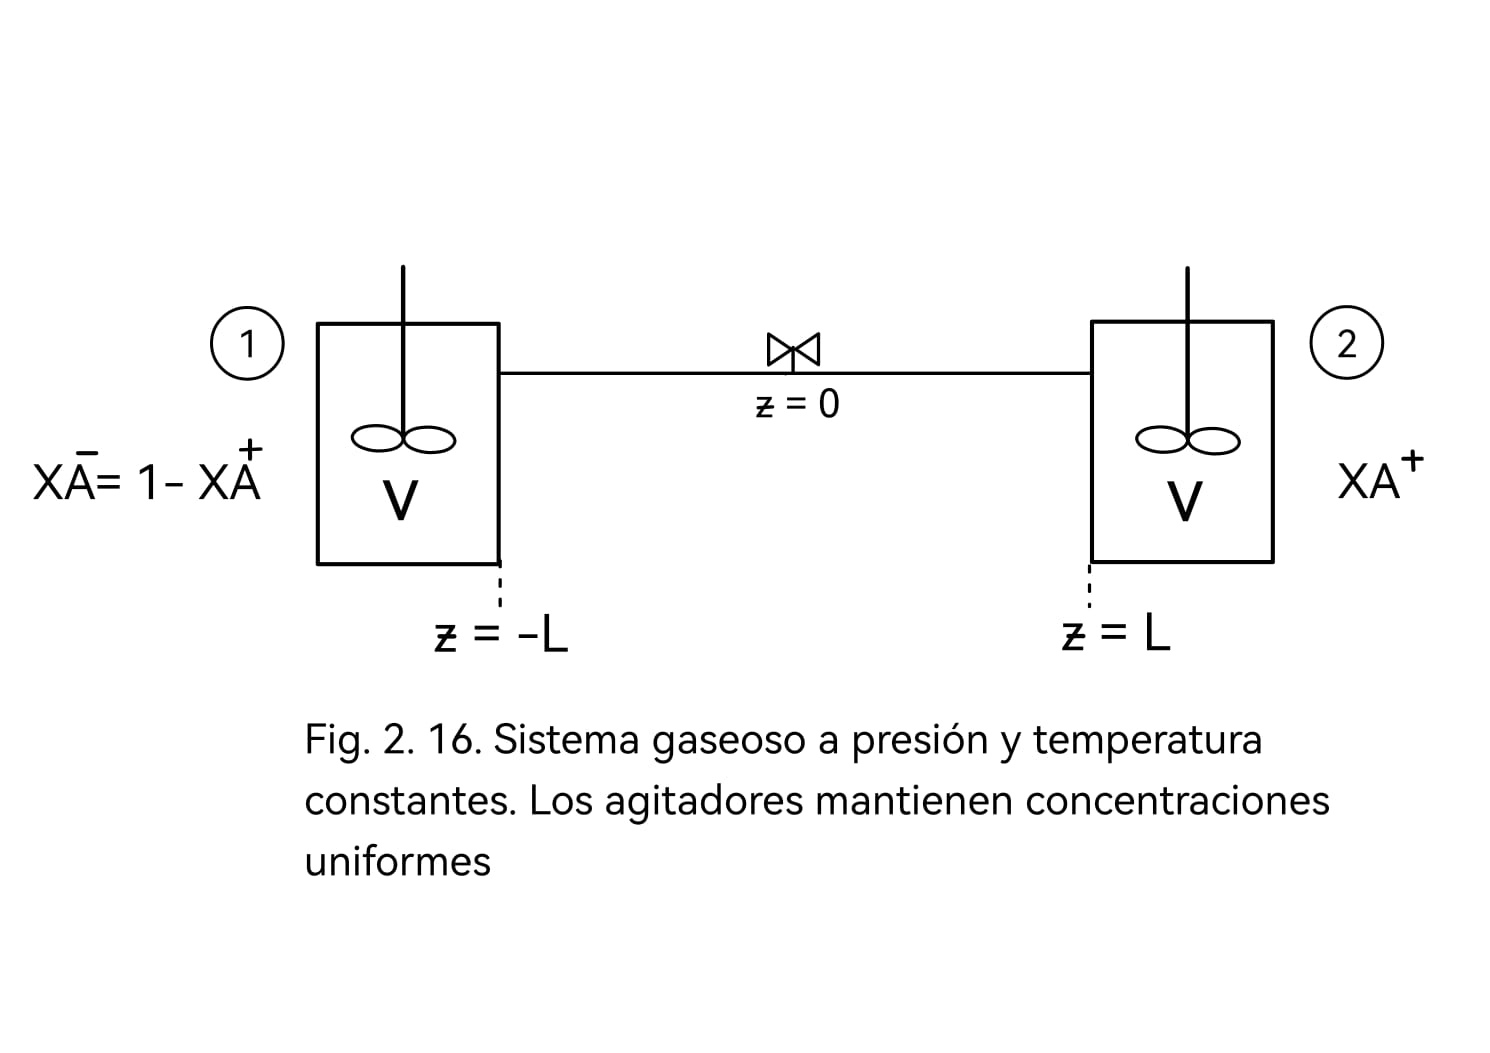
\includegraphics[width=\linewidth]{./Capitulo2/Imagenes/imagen-4.jpg} % Imagen ajustada al bloque
\end{minipage}
\hfill % Espaciado entre imagen y texto
\begin{minipage}{0.45\textwidth} % Tamaño del bloque del texto
El aparato tiene un gas A en el recipiente \textbf{1} y un gas B en el recipiente \textbf{2}.  La válvula se abre y la difusión comienza.  Se mide $x_A$ en función del tiempo, lo que permite medir $\mathscr{D}_{AB}$.
\end{minipage}

\textbf{Las condiciones de frontera son:} \quad
$
x_A \bigg|_{Z=-L}= x_A^- \quad \ y \quad x_A \bigg|_{Z=L}= x_A^+ \quad
$

\textbf{Calcular lo siguiente}
\flushleft
(a)- Mostrar que $N_A$ es constante.
\flushleft
(b)- Mostrar que el flujo de masa es:\quad $ N_{A Z}= - c \mathscr{D}_{AB} \frac{dx_A}{dz} $
\flushleft
(c)- Integrar la ecuación.
\flushleft
(d)- Evaluar la constante de integración.
\flushleft
(e)- Obtener:\quad 
$ N_{AZ} = \frac{(\frac{1}{2}-x_A^+)c\mathscr{D}_{AB}} {L}$
\flushleft
(f)- Hacer un balance de masa en el recipiente 2 para obtener:\quad 
   $ S(\frac{1}{2}-x_A^+)\frac{c\mathscr{D}_{AB}} {L} = V_c 
   \frac{dx_A^+}{dt} $
\flushleft
(g)- Integrar la ecuaciónpara obtener: \quad
$
\ln (\frac{\frac{1}{2}-x_A^+}{\frac{1}{2}})=\frac{-S\mathscr{D}_{AB}t}{LV}
$
\flushleft
(h)- Hacer una gráfica para obtener $\mathscr{D}_{AB}$ 
\vspace{0.2cm}
\newpage
\textbf{3. Difusión desde una gota suspendída.} \textit{(Problema. 18.B.7. Bird et al.)}
\flushleft
\begin{minipage}{0.45\textwidth} % Tamaño del bloque de la imagen
    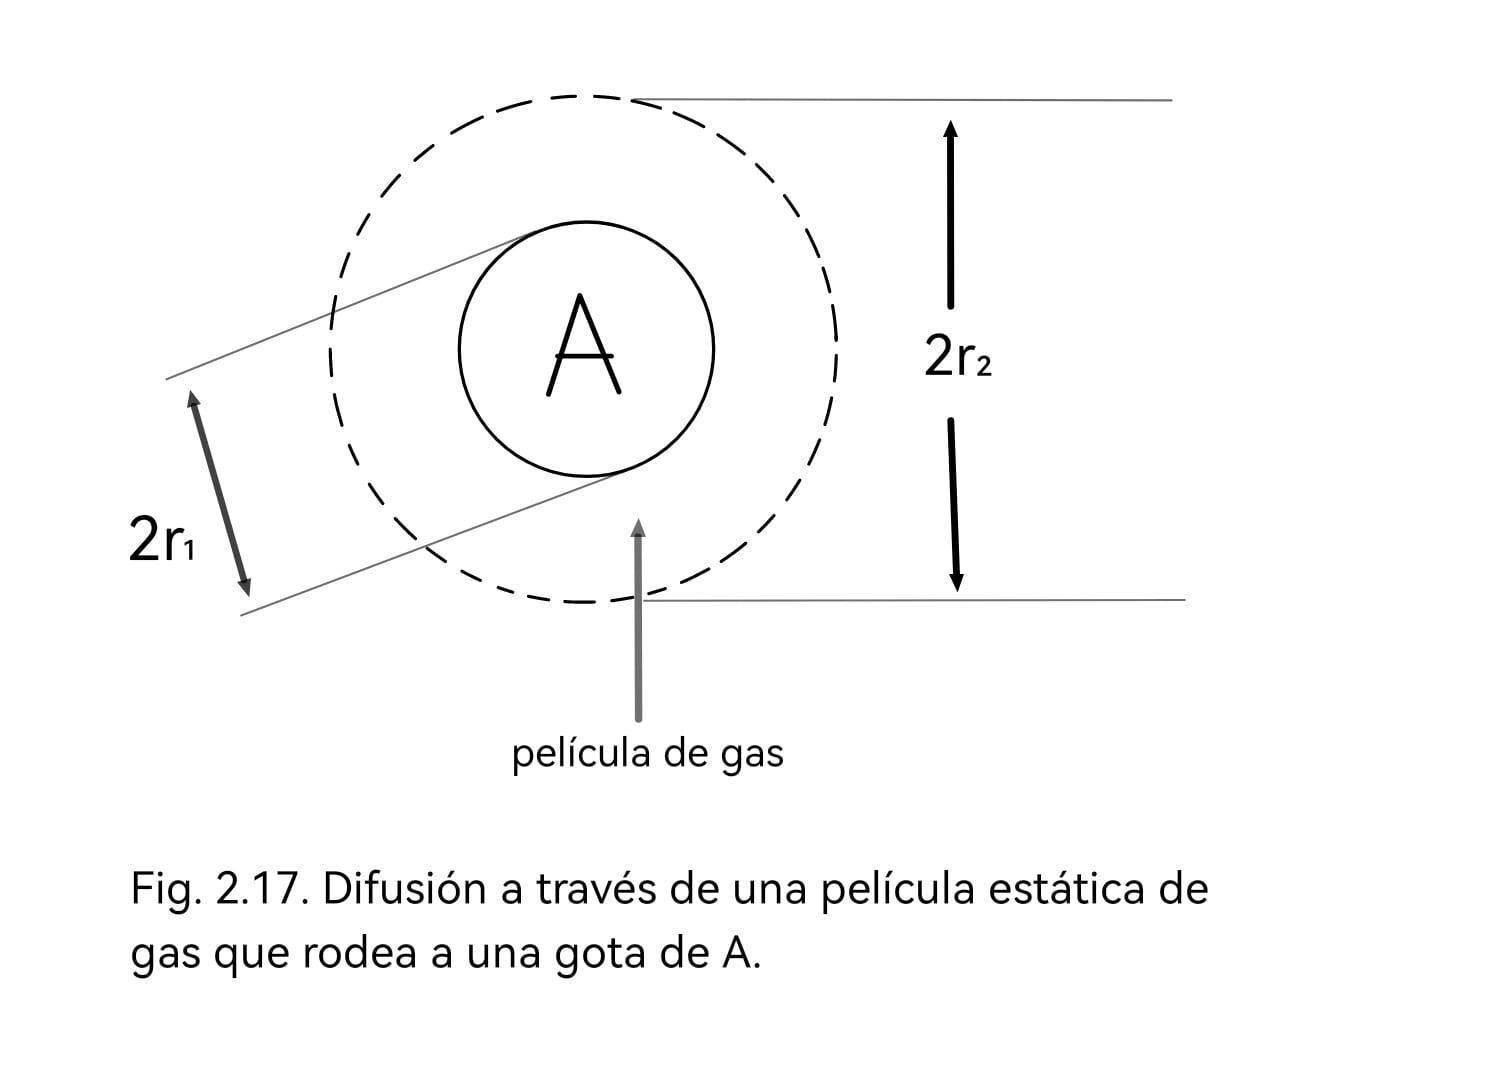
\includegraphics[width=\linewidth]{./Capitulo2/Imagenes/imagen-6.jpg} % Imagen ajustada al bloque
\end{minipage}
\hfill % Espaciado entre imagen y texto
\begin{minipage}{0.5\textwidth} % Tamaño del bloque del texto
Una gota de líquido A de radio $r_1$ está suspendída en una corriente de gas B. Supóngase la presencia de una película alredesor de la gota de radio $r_2$. La concentración de A en la fase gas en $x_A$, en r=$r_1$ y $x_A2$ en r=$r_2$.
\end{minipage}
Demuestra:
\flushleft
(a)- Que $r^{2}N_Ar$ es constante ene la fase gas.Evaluar la constante en r=$r_1$ para obtener $r^{2}_1N_Ar$, en la superficie de la gota:
\flushleft
(b)- La ecuacíon (1.25) y el resultado anterior resulta en: \[r^{2}_1N_Ar_1=\frac{-c\mathscr{D}_{AB}}{1-x_A}r^{2}\frac{dx_A}{dr}\]
(c)- La integración entra $r_1$ y $r_2$ resulta en:
\[ N_{Ar_1}=\frac{c\mathscr{D}_{AB}}{r_2-r_A1}(\frac{r_2}{r_1}){\ln {\frac{x_{B2}}{x_{B1}}}}\]
(d) Obtener el límite de esta ecuacíon cuando $r_2\rightarrow \infty$.
\newpage
\section*{Tarea 4}

\textbf{1. Absorción de cloro en ciclohexeno.} \textit{(Problema. 18.B.5 Birt et al.)}
\flushleft
El cloro se puede absorber de una mezcla Cl$_2$-aire por medio de olefinas disueltos en CCl$_4$. La reacción de Cl$_2$ con ciclohexano (C$_{6}$H$_{10}$) es de segundo orden con respecto al cloro y de orden cero con respecto al C$_{6}$H$_{10}$. Por lo tanto, la desaparición de cloro por unidad de volumen es $k_2 C_A^2$ ( $A = \text{Cl}_2$).
\flushleft
Modificar el problema de la sección (2.3) donde $B =$ C$_{6}$H$_{12}$-CCl$_4$, suponiendo que la reacción puede pseudobinaria. Suponer que el aire es insoluble en $B$ y que $L \to \infty$.
\flushleft
(a)- Demostrar que el perfil de concentraciones está expresado como:
 \[ 
 \frac{C_{A0}}{C_{A}} = \left[1 + \sqrt{\frac{k_2 C_{A0}}{6\mathscr{D}_{AB}}} Z \right]^{-}
    \]
(b)- Obtener la rapidez de absorción de Cl$_2$ por el líquido.
\flushleft
(c)- Suponiendo que $A$ se disuelve y reacciona con $B$, de tal forma que la rapidez de desaparición de $A$ es una función de la concentración f($B_A$). Mostrar que el flux de masa de $A$ es:
\[
N_{A2} \bigg|_{z=0} = \sqrt{2 \theta_{A0} \int_{0}^{C_{A0}} f(C_A) \, dC_A}
\]
Usa este resultado para verificar (b)
\flushleft
\textbf{2.  Difusión con reacción química de segundo orden}\textit{(Problema 18.B.11. Bird et al.)}
\flushleft
El sólido $A$ se disuelve en una corriente $S$ líquida isotérmicamente. De acuerdo con el modelo de la película (sección 2.1.1), la superficie de $A$ está cubierta por una película de líquido estática de grosor $\delta$ (Fig. 2.2).

(a)- Desarrollar una expresión de la rapidez de disolución de $A$ en $S$ si la concentración de $A$ en $S$ es pequeña.

(b)- Si $S$ contiene una sustancia $B$, tal que en el plano $z = k\delta$ reacciona con $A$ ($A + B \to P$). Por ejemplo, la disolución de ácido benzoico en una solución de NaOH. La corriente de líquido consiste en $S + B$, donde la fracción mol de $B$ es $x_{B\infty}$ (Ver Fig. 2.18). 
Es necesario suponer que $A$ y $B$ se difunden a través de una capa pequeña . (zona de reacción en la Fig. 2.18)
\begin{figure}[h]
    \centering
    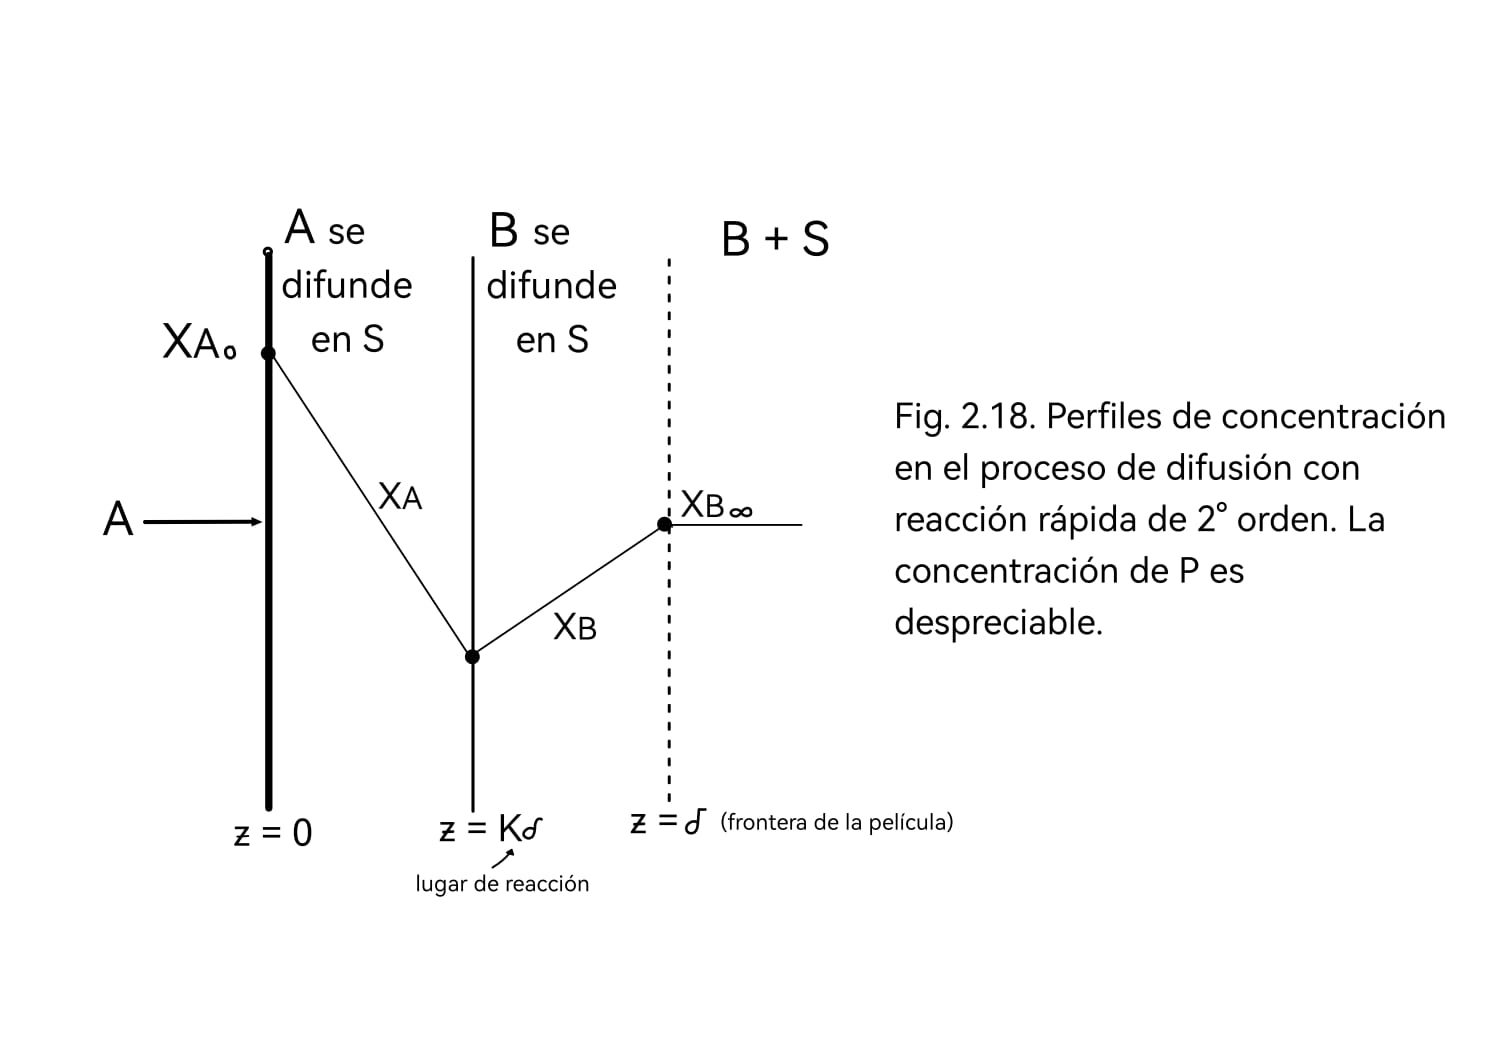
\includegraphics[width=0.5\textwidth]{./Capitulo2/Imagenes/imagen-8.jpg} 
    \label{fig:etiqueta}
\end{figure}
\flushleft
\textit{Respuesta:}
\flushleft
(a)-\quad $
N_{Az} \bigg|_{z= D}=\frac{c\mathscr{D}_{AS}x_{A_D}}{\delta} 
$
\flushleft
(b)-\quad $
N_{A2} \bigg|_{z=D}=\frac{c\mathscr{D}_{AS}x_{A_D}}{\delta}(1+\frac{x_{BD}D_{BS}}{x_{AD}\mathscr{D}_{AS}})
$
\newpage
\textbf{3. Demanda de oxígeno por agregados de bacterias}\textit{(Problema 18.B.19. Bird et al.)}
\flushleft
Supongan un agrergado de bacterias esferico de R. Se desea determina la demanda de $O_2$ del agregado como función su tamaño, concetración de $O_2$ ($\rho_0$) en la superficie del agregado, la actividad metabólica de la células y el comportamientos difusinal del $O_2$. Supone que la difusión de $0_2$ está expresada como $r_{O_2}=-k_0$ y el comportamiento difusional esta gobernado por la ley de Fich condifusividad $D_{\upsilon_2m}$
\flushleft
(a)-Demostrar que el perfil de concentración de $O_2$ se describe por medio de la siguiente ecuación:
\[
\frac{1}{\xi^{2}}\frac{d}{d\xi}(\xi^{2}\frac{dx}{d\xi})= N \quad \text{donde} \quad X=\frac{\rho_{02}}{\rho_0},\quad  \xi=\frac{r}{R} \quad y \quad \nu= \frac{k_R^{2}}{\rho_0D_{O_2m}}
\]
(b)- Si $N$ es grande, tal que $x=0$ para $\xi<\xi_0$, existe zona central en el agregado sin $O_2$. Se reconoce que $X$ y $\frac{dX}{d\xi}$ son cero en $\xi=\xi_0$. ¿Cual es el significado físico de estos suposiciones?
\flushleft
(c)- Integrar la ecuación anterior con las condiciones de frontera propicios.
\flushleft
\textit{Respuesta:}
\[
x= 1 -\frac{N}{6}(1-\xi^{2})+\frac{N}{\xi}\xi^{2}_0(\frac{1}{\xi}-1) \quad  donde \quad \xi_0 \quad \text{es determinado por la siguiente ecuación:}\quad \xi^{3}_0-\frac{3}{2}\xi^{2}_0 +(\frac{1}{2}-\frac{3}{\xi})=0
\]
\newpage
\section*{Tarea 5}
\textbf{1. Difusión y reacción heterogenea en el tubo con un extremo cerrado.} \textit{(Problema. 18.B.15 Birt et al.)}
\flushleft
\begin{minipage}{0.4\textwidth} % Tamaño del bloque de la imagen
    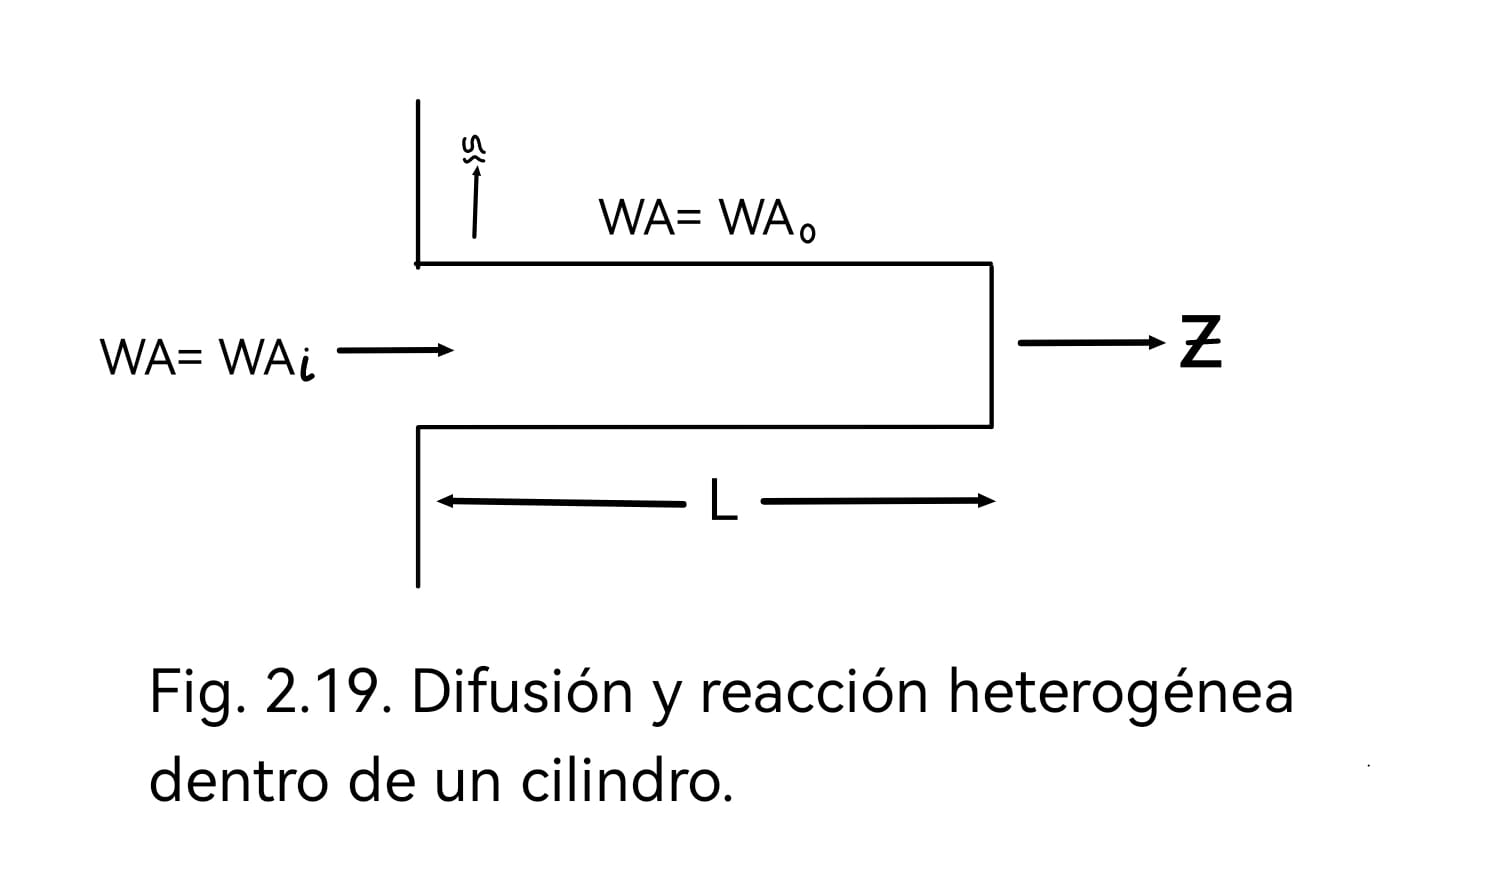
\includegraphics[width=\linewidth]{./Capitulo2/Imagenes/imagen-7.jpg} % Imagen ajustada al bloque
\end{minipage}
\hfill % Espaciado entre imagen y texto
\begin{minipage}{0.5\textwidth} % Tamaño del bloque del texto
Un poro cilíndrico de longitud \( L \) y sección \( S \) está en contacto con un fluido en su extremo abierto. El fluido contiene \( A \) y \( B \),  en donde \( A \) desaparece dentro del poro, se difunde a lo largo y reacciona sobre las paredes. El flux normal a la superficie es función de la fracción masa \( W_{AU} \) de \( A \) sobre la superficie y depende de \( z \). La temperatura y densidad son constantes, ya que la concentración de \( A \) es pequeña. Como el poro es largo, los gradientes de concentración normales a \( z \) son pequeños.
\end{minipage}
\flushleft
(a)-  Mostrar que el régimen es permanente.\quad
$
\frac{dWA}{dz} = \frac{P}{S} f(WA)
$
\flushleft
(b)- Demostrar que la velocidad promedio másica \( V_{z} \) es cero para este sistema.
\flushleft
(c)- Sustituir la ley de Fick \( J_A = -\rho \mathscr{D}_{AB} \nabla WA \) en la ecuación anterior e integrar la expresión resultante para el caso \( f(WA) = k_iW_{A_0} \).  La condición de frontera en \( z = L \) supone que no hay reacción en ese extremo.
\flushleft
(d)- Desarrolla una expresión para \( W_A \) en el cilindro.
\flushleft
\textit{Respuesta:}
\flushleft
(c)- \quad$
    \frac{WA}{WA_i} = \frac{\cosh N \left[1 - \frac{z}{L}\right]}{\cosh N} \quad donde \quad N=\sqrt{\frac{PL^{2}k_1}{S{\rho}\mathscr{D}_{AB}}}
    $
\flushleft
(d)- \quad$ W_A=(\frac{S{\rho}\mathscr{D}_{AB}W_{Ai}}{L})N \tan{h}N $
\flushleft
\vspace{0.5cm} 
\textbf{2. Cálculo de la longitud de un reactor isotérmico.}\textit{(Problema 18.C.4 - Bird et al.)}
\flushleft
Sea \( a \) el área de la superficie de un catalizador y \( S \) la sección del reactor. Suponer que el flujo másico es \( w \) (en \(\text{lbm}/\text{hr}\)).
\flushleft
(a)- Mostrar que el balance a régimen permanente de \( A \) a una distancia \( L \) está dado por:
 \[
    \frac{dW_{A_0}}{dL} = - S a N A
    \]
(b)- Utilizar la ecuación (2.74) y el resultado anterior para obtener una expresión de la longitud \( L \) necesaria para convertir la composición a la entrada \( X_A(0) \) en la de la salida \( X_A(L) \). Utilizar la relación:\quad
    $
    \gamma_\alpha = M_\alpha N_\alpha
    $
\flushleft
\textit{Respuesta:}
  \[
    L = \frac{w \delta M_B}{25 a c\mathscr{D}_{AB}} \int_{X_A(0)}^{X_A(L)} \frac{dX_{A_0}}{\left[ {M_A X_{A_0} + M_B (1 - X_{A_0})} \right]^2 \ln \left( 1 - \frac{1}{2} X_{A_0} \right)}
    \]
\flushleft
\vspace{0.5cm} 
\textbf{3. Difusión y reacción química en un líquido}\textit{(Problema 19.B.6 - Bird et al.)}
\flushleft
(a)- Una esfera sólida de \( A \) está suspendida en un líquido \( B \) en el que \( A \) es ligeramente soluble y en donde \( A \) reacciona con constante cinética. Mostrar que el perfil de concentraciones es:
\[
    \frac{C_A}{C_{A_s}} = \frac{R}{r} \frac{e^{-b\frac{r}{R}}}{e^{-b}}, \quad b^2 = \frac{k_1R^{2}}{\mathscr{D}_{AB}}
    \]
 \( R \) es el radio de la esfera y \( C_{A_s} \) es la solubilidad molar de \( A \) en \( B \).
 \flushleft
 (b)-  En régimen cuasiestático, calcular la disminución del diámetro de la esfera a medida que se disuelve y reacciona.  Mostrar que la relación radio/ tiempo en: 
   \[
    \sqrt{\frac{k_1}{\mathscr{D}_{AB}}} (R - R_0) - \ln \frac{1 + \sqrt{\frac{k_1}{\mathscr{D}_{AB}}} R}{1 + \sqrt{\frac{P_B}{\mathscr{D}_{AB}}} R_0} = -\frac{k_1 C_{A_0} M_A (t - t_0)}{\rho_s}
    \]
en donde \( R_0 \) es el radio de la esfera en \( t_0 \) y \( \rho_s \) es la densidad de la esfera.
\newpage
\section*{Tarea C}

\textbf{1. Factor de efectividad en discos delgados} \textit{(Problema 18.B.14 - Bird et al.)}
\flushleft
\begin{minipage}{0.4\textwidth} % Tamaño del bloque de la imagen
    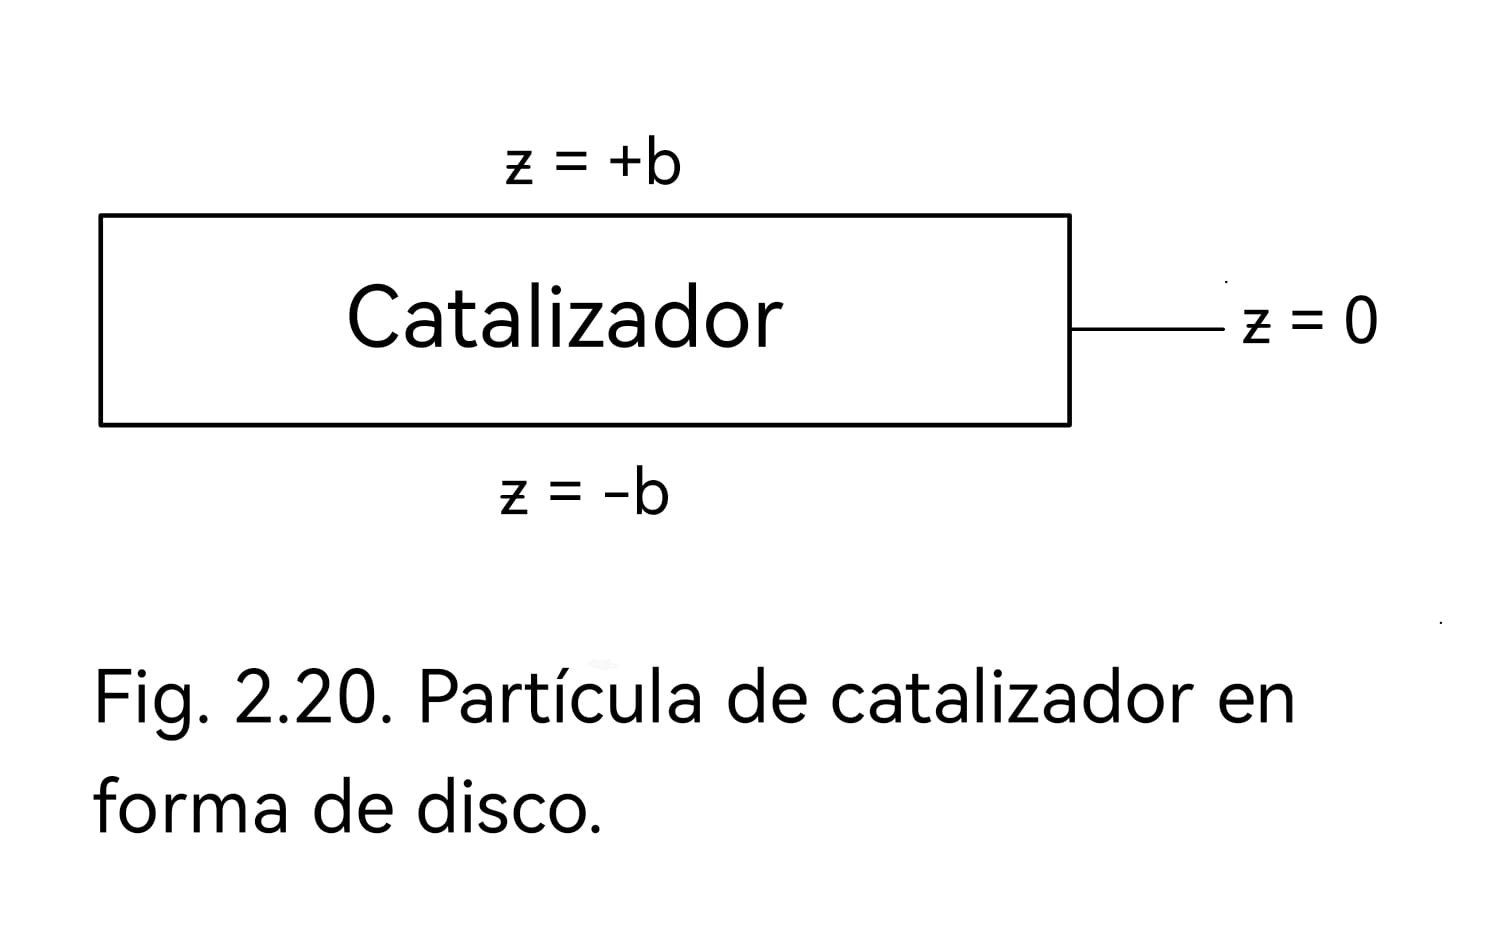
\includegraphics[width=\linewidth]{./Capitulo2/Imagenes/imagen-5.jpg} % Imagen ajustada al bloque
\end{minipage}
\hfill % Espaciado entre imagen y texto
\begin{minipage}{0.55\textwidth} % Tamaño del bloque del texto
Considerar en este caso que el área del grosor del disco es muy pequeña en comparación con el área de los discos. Demostrar que el perfil de concentraciones es:
\end{minipage}
\[
 \frac{C_A}{C_{A_s}} = \frac{\cosh \left(\frac{\lambda}{\mathscr{D}_{AB}} z\right)}{\cosh \left(\frac{\lambda}{\mathscr{D}_{AB}} b\right)}
    \]
Mostrar que el flujo másico en las superficies \( z = \pm b \)  es:
\[
    |W_A| = 2 \pi R^2 C_{A_s} \mathscr{D}_{AB} \lambda \tanh \lambda b, \quad \lambda=\sqrt{\frac{k_1a}{D_A}}
\]

Mostrar que si el disco es cortado paralelo al plano \( x-y \) en varios  cortes o rebanadas $n$, el flujo másico total sería:
\[
    |WA^{(n)}| = 2 \pi R^2 C_{A_s} \mathscr{D}_{AB} \lambda n \tanh \left(\frac{\lambda b}{n}\right)
    \]
Obtener la expresión del factor de efectividad tomando el límite:
    \[
    \eta_A = \lim_{n \to \infty} \frac{|WA|}{|WA^{(n)}|} = \frac{\tanh (\lambda b)}{\lambda b}
    \]
    
















\chapter{Capítulo 3}
Capa Límite con Difusión, Dispersión de Taylor y Flujo Turbulento con Difusión.

Este capítulo consta de las siguientes partes:
\begin{enumerate}
    \item Capa límite.
    \item Convección forzada con reacción química homogéna en una placa plana.
    \item Convección forzada  placa plana con transferencia de masa rápida.
    \item Convección forzada  placa plana con transferencia de masa lenta.
    \item Dispersión de Tayloren flujo laminar.
    \item Transferencia de masa con reacción de $1^{\text{er}}$ orden en flujo laminar turbulento.
    \item Flujo turbulento en reacción de $2^{\circ}$ orden. Mezclado turbulento.
\end{enumerate}
\section{Capa límite binaria}
Considerar un flujo binario a régimen permanente de un fluido binario. En la vecindad de la superficie sólida, las ecuaciones que gobiernan el proceso en ausencia de disipación viscosa son:
 \begin{equation}
\text{Continuidad: }\frac{\partial v_x}{\partial x} + \frac{\partial v_y}{\partial y} = 0 \label{3.1}
\end{equation}
\begin{equation}
    \begin{split}
    \text{Movimiento: } &\rho \left( v_x \frac{\partial v_x}{\partial x} + v_y \frac{\partial v_x}{\partial y} \right) =- \rho v_e \frac{\partial v_e}{\partial x} + \mu \frac{\partial^2 v_x}{\partial y^2} \\
    & + \bar{\rho} g_x \beta (T - T_{\infty}) + \bar{\rho} g_x \bar{\zeta} (w_A - w_{A\infty})
    \end{split}
    \label{3.2}
\end{equation}
\begin{equation}
    \text{Energía: } \rho \bar{C_p} \left( v_x \frac{\partial T}{\partial x} + v_y \frac{\partial T}{\partial y} \right) = 
    k \frac{\partial^2 T}{\partial y^2} - \left( \frac{\bar{H}_A}{M_A} - \frac{\bar{H}_B}{M_B} \right) r_A
    \label{3.3}
\end{equation}
\begin{equation}
    \text{Continuidad de A: } \rho \left( v_x \frac{\partial w_A}{\partial x} + v_y \frac{\partial w_A}{\partial y} \right) = 
    \rho \mathscr{D}_{AB}  \frac{\partial^2 w_A}{\partial y^2} + r_A 
    \label{3.4}
\end{equation}
donde $v_e$ es la velocidad en el límite externo de la capa límite de velocidad, $T_{\infty}$ es la temperatura en el límte externo de la capa límite térmica y $w_{A\infty}$ es la concentración másica en el límite externo de la capa límite difusional.
Los términos de flotación en la ec.(\eqref{3.2}) provenien del efecto témrico y del de concentración. En la ec.\eqref{3.3} se incluye el término de fuente de calor por reacción química. Las ecs.\eqref{3.1}-\eqref{3.4} pueden ser integrados para dar

Ecs. continuidad+movimiento:
\begin{equation}
    \begin{split}
    \mu \frac{du_x}{dy} \bigg|_{y=0} = &\frac{d}{dx} \int_{0}^{\infty} \rho v_x (v_e - v_x) dy + \frac{d v_e}{dx} \int_{0}^{\infty} \rho (v_e - u_x) dy + \rho v_o v_e + \\
   &- \int_{0}^{\infty} \rho g_x \beta (T - T_{\infty}) dy  - \int_{0}^{\infty} \rho g_x \bar{\zeta} (w_A - w_{A\infty}) dy
    \label{3.5}
\end{split}
\end{equation}

Ecs. continuidad+energía:
\begin{equation}
    k \frac{dT}{dy} \bigg|_{y=0} = \frac{d}{dx} \int_{0}^{\infty} \rho v_x \bar{C_p} (T_{\infty} - T) dy
    - \int_{0}^{\infty} \left( \frac{\bar{H}_A}{M_A} - \frac{\bar{H}_B}{M_B} \right) r_A dy
    - \rho v_{\infty} \bar{C_p} (T_{\infty} - T_0) 
    \label{3.6}
\end{equation}

Ecs. continuidad+continuidad de A:
\begin{equation}
    \rho \mathscr {D}_{AB} \frac{dw_A}{dy} \bigg|_{y=0} = \frac{d}{dx} \int_{0}^{\infty} \rho u_x (w_{A\infty} - w_A) dy
    + \int_{0}^{\infty} r_A dy - \rho v_{0} (w_{A\infty} - w_{A0})
    \label{3.7}
\end{equation}

Estas ecuaciones son extensiones de los balances de von Kármán y de la integral de momentum expuestas en el libro 1, Cap. 5.

\section{Convección forzada con reacción química homogénea en una placa plana}
\section{Convección forzada en placa plana con transferencia de masa rápida}
\section{Convección forzada en placa plana con transferencia de masa lenta}
\section{Difusión de Taylor en flujo laminar}
\section{Transferencia de masa con reacción de $1^{er}$ orden en flujo turbulento}


\section{Flujo Turbulento con Reacción de Segundo Orden. Mezclado Turbulento}

Considerar dos casos en los que existen dos solutos $A$ y $B$ disueltos en un solvente $S$. En el primer caso no existe reacción, y en el segundo caso se produce la reacción:
\begin{equation*}
    A + B \rightarrow \text{productos}
\end{equation*}
En ambos casos se estudia el mezclado turbulento en dos sistemas: mezclador estático (a) y dinámico (b).

\begin{figure}[h]

        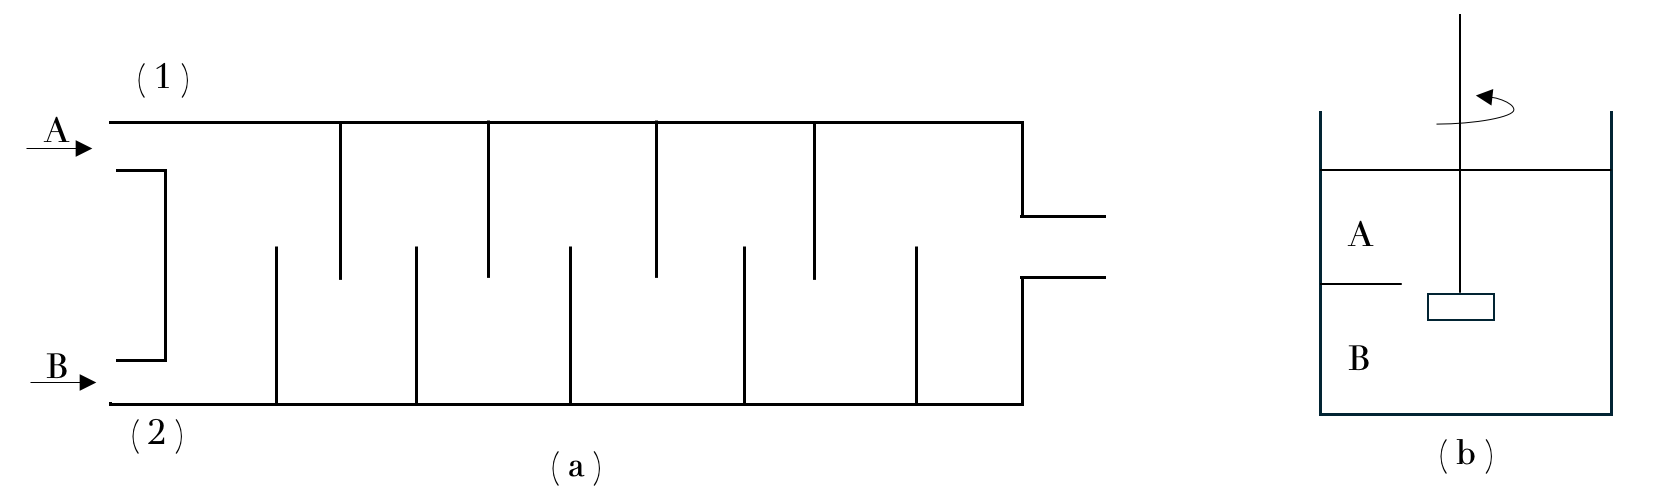
\includegraphics[width=\linewidth]{Capitulo3/Imagenes/Fig_3.8.png}
        \caption{Mezclador estático (a) y mezclador dinámico (b)}
        \label{fig:Fig_3.8}

\end{figure}
        El comportamiento de los solutos A y B se describe por medio de las siguientes ecuaciones de difusión:




\begin{equation}
    \frac{\partial C_A}{\partial t} + \underline{v} \cdot \nabla C_A = \mathscr{D}_{AS} \nabla^2 C_A + R_A
    \notag
\end{equation}

\begin{equation}
    \frac{\partial C_B}{\partial t} + \underline{v} \cdot \nabla C_B = \mathscr{D}_{BS} \nabla^2 C_B + R_B
    \label{eq_3.82}
\end{equation}




Condiciones de frontera:

\begin{equation}
    C_A = C_{A0}, \quad C_B = 0 \quad \text{para } z=0, t=0
    \notag
\end{equation}

\begin{equation}
    C_B = C_{B0}, \quad C_A = 0 \quad \text{para } z=0, t=0
\end{equation}

\subsection{Sin Reacción}

Definiendo:
\begin{equation}
    \Gamma = \frac{C_{A0} - C_A}{C_{A0}} = \frac{C_B}{C_{B0}}
\end{equation}

Las ecuaciones \eqref{eq_3.82} se reducen a:

\begin{equation}
    \frac{\partial \Gamma}{\partial t} + v \cdot \nabla \Gamma = D_{is} \nabla^2 \Gamma
\end{equation}

En las entradas (1) y (2):

\begin{equation}
    \Gamma_1 = 0, \quad \Gamma_2 = 1 \notag
\end{equation}

En flujo turbulento se propone que:

\begin{equation}
    \Gamma = \bar{\Gamma} + \Gamma'
\end{equation}

donde:
\begin{equation}
   \bar{\Gamma} = \frac{C_{A0} - \bar{C}_A}{C_{A0}} = \frac{\bar{C}_B}{C_{B0}}
\end{equation}




y $\Gamma'$ (grado de ausencia de mezclado). Restando $\Gamma$ - $\bar{\Gamma}$  y efectuando el cuadrático medio:

\begin{equation}
    \left( \frac{C_A}{C_{A0}} \right)^2 - \left( \frac{\bar{C}_B}{C_{B0}} \right)^2 = d^2
\end{equation}

En donde $d^2$ es la función de decaimiento que tiende a cero a distancias $z$ grandes o tiempos largos.


La administración de la función de decaimiento indica su dependencia funcional. Definiendo la longitud y velocidades características $l_{0}$ y $v_{0}$, obtuvimos:

\begin{equation}
    \frac{\partial\Gamma}{\partial t} + v_{b}\hat{\nabla}\Gamma = \frac{1}{Re Sc}\hat{\nabla}^{2}\Gamma  \label{eq_3.89}
\end{equation}


donde 

\begin{equation}
      \hat{t}=\frac{v_0t}{l_0}, \quad 
      \hat{v}=\frac{v}{v_0},\quad
      \hat{\nabla}=l_0\nabla, \quad
       Re=\frac{l_0v_0}{\mu}\rho 
\end{equation}

En el caso de tanques de mezclado, $l_0$ es el diámetro del impulson, $v_0=l_0N$ (N es la velocidad angular). En el caso del mezclado de dos corrientes de tubos concéntriccos \eqref{fig:Fig_3.9}, la función de decaimiento resultante se grafica en función de la distnacia axial. El mezclado a nivel molecular (micromezclado) se alcanza

\begin{figure}[h]

        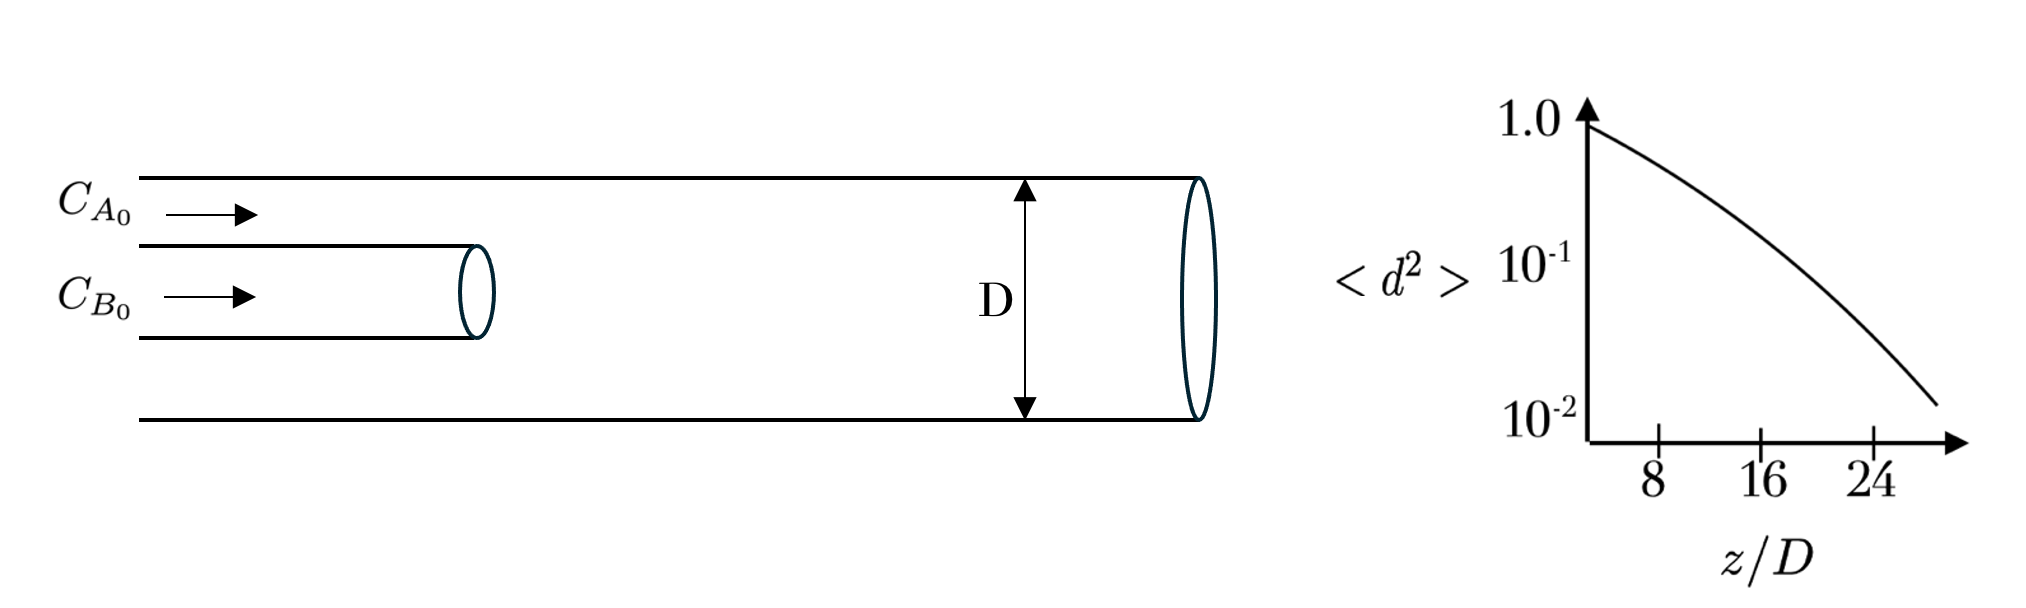
\includegraphics[width=\linewidth]{Capitulo3/Imagenes/Fig_3.9.png}
        \caption{Mezclado de 2 corrientes de A y B en tubos concéntricos y su función de decaimiento}
        \label{fig:Fig_3.9}

\end{figure}

En procesos industriales, normalamente $ReSc\sim10^9$, por lo que la ecuación \eqref{eq_3.89} se reduce a:


\begin{equation}
    \frac{\partial\Gamma}{\partial t} + v_0\hat{\nabla}\Gamma = 0
\end{equation}


Por lo que el grado de mexclado depende de $\hat{t}$ y no de $ReSc$. Como $\hat{t}=Nt_{mix}$, el producto del tiempo de mezclado $t_{mix}$ por la velocidad angular es constante, independiente de $Re$, o sea, $Nt_{mix}=K$, donde K depende de la geometría solamente.

\subsection{Con Reacción}
\begin{equation*}
    A + B \rightarrow \text{productos}
\end{equation*}
Definiendo
\begin{equation}
    \Gamma_{r}=\frac{C_{A0}-(C_A-C_B)}{C_{A0}+C_{B0}}
\end{equation}
Por la resta de las ecuaciones \eqref{eq_3.82}, la descripción del caso con reacción es la misma. Por ello:
\begin{equation}
    \left[ \frac{C_{A0}-(C_A-C_B)}{C_{A0}+C_{B0}} \right]_{reac.}=   \left[ \frac{C_{A0}-C_A}{C_{A0}}\cdot\frac{C_B}{C_{B0}} \right]_{\text{sin reac.} }
\end{equation}
que tambien es válida para las fluctuaciones.
\begin{equation}
        \left[ \frac{C_A'-C_B'}{C_{A0}+C_{B0}} \right]_{reac.}=  \left[ \frac{C_A'}{C_{A0}} \right]_{\text{sin reac.} }
\end{equation}

Esta ecuación sugiere que las fluctuaciones en $C_A$ y $C_B$ en problemas con reacción tienen lugar al mismo tiempo y escalas de distancia que los problemas sin reacción. Los casos particualres son:
\par
a) Reacción rápida: La velocidad de la reacción es controlada por difusión de las especies. Durante la escala del micromezclado, en la que la difusión es lenta en comparación con la convección, el efecto de la reacción es pequeño. En este caso tenemos:
\begin{equation}
            \left( \frac{C_A'}{C_{A0}} \right)_{reac.}=  \left( \frac{C_A'}{C_{A0}} \right)_{\text{sin reac.} }
\end{equation}
En la práctica, las reacciones rápidas son empleadas para determinar la eficiencia de los mezlcados.
\par
b) Reacciones lentas: Considerar el caso de reacciones de segundo orden irreversibles.
\begin{equation}
    R_A=-k_2C_AC_B
\end{equation}
Promediando en el tiempo: 
\begin{equation}
    R_A=-k_(\bar{C_A}\bar{C_B}+C_A'C_B')
\end{equation}
Esto indica que las fluctuaciones en $C_A$ y $C_B$ incrementan la velocidad de reacción. Por medio de un análisis de órdenes de magnitud, tenemos:
\begin{equation}
    t_A=\frac{C_{A0}}{R_A}\sim\frac{1}{k_2C_{B0}}
\end{equation}
Para una reacción rápida $t_{mix}>>t_A$ \newline
Para una reacción lenta $t_{mix}<<t_A$



\newpage
\section* {Apéndice A}
a) Transferencia de masa lenta en una placa plana. Uso de la ecuación \textbf{HACER REFERENCIA A LA ECUACIÓN 3.46}
\newline

Estimación de la velocidad de evaporación, $u_{A0}$, como función de $Sc$, del secado de una placa plana porosa saturada de agua \textbf{HACER REFERENCIA A LA FIGURA 3.2} por medio de una corriente de aire bajo condiciones tal que $W_{A0}=0.05$, $W_{A0}=0.01$ y $Sc=0.6$.
\newline
La ecuación \textbf{HACER REFERENCIA A LA ECUACIÓN 3.46} es:
\begin{equation*}
    \frac{j_{A0}}{\rho v_o(w_{A0}-w_{A\infty})}Sc^{2/3}=0.332\sqrt{\frac{\nu}{v_\infty x}}
\end{equation*}
Por medio de las ecuaciones \eqref{eq_1.24}: $n_{B0}=w_{A_0}(\underline{n}_{A_0}+\underline{n}_{B_0})+\underline{j}_{A_0}$ ya que $\underline{n}_{B_0}=0$, sustituyendo esta ecuación en la \textbf{HACER REFERENCIA A LA EC 3.46}

\begin{equation*}
    \frac{n_{A_0}(1-w_{A_0})}{\rho v_\infty (w_{A_0 }-w_{A\infty)}}=0.332Sc^{-2/3}\sqrt{\frac{\gamma}{v_\infty x}}
\end{equation*}

\begin{equation*}
n_{A_0}=0.332Sc^{-2/3}\frac{(w_{A_0}-w_{A_\infty})}{1-w_{A_0}}\rho v_\infty\sqrt{\frac{\mu}{v_\infty x \rho}}=(0.332)(0.6)^{-2/3}\frac{(0.05-0.01)}{1-0.05}\sqrt{\frac{\rho v_\infty \mu}{x}}
\end{equation*}
\begin{equation*}
    n_{A_0}=0.0196 \sqrt{\frac{\rho v_\infty \mu}{x}}
\end{equation*}
\par
b) Transferencia de momentum, calor y masa simultáneos
\newline
Las ecuaciones \textbf{HACER REFERENCIA A LA EC 3.43} y \textbf{EC 3.44} se pueden generalizar para incluir la transferencia de calor:
\begin{equation}
    \frac{q_0}{\rho \hat{C}pv_\infty(T_0-T_\infty)}=\frac{f''(0)}{Pr}\sqrt{\frac{J}{2v_\infty x}}
    \tag{A-1}
    \label{eq_A-1}
\end{equation}
Las ecuaciones \eqref{eq_A-1}, \textbf{HACER REFERENCIA A LA EC 3.43 3.44} se pueden utilizarse en las transferencias simultáneas generalizando la expresión de k \textbf{HACER REFERENCIA A LA EC 3.38}

\begin{equation}
    K=\frac{\rho_0 v_0 (x)}{\rho v_\infty}\sqrt{\frac{2v_\infty x}{\gamma}}
    \tag{A-2}
    \label{eq_A-2}
\end{equation}
donde $\rho$, $\mu$, $\hat{C}p$ y $\mathscr{D}_{AB}$ sean evaluadas a las condiciones de referencias siguientes: $T_f=\frac{1}{2}(T_0+T_\infty)$ y $W_{Af}=\frac{1}{2}(W_{A_0}+W_{A\infty})$
\newline
La resolución de problemas de transferencia simultáneas se facilita por medio de las siguientes relaciones de los fluxes:

\begin{equation*}
   R_v=\frac{(n_{A_0}+n_{B_0})(v_\infty-e)}{\tau_0} 
\end{equation*}

\begin{equation}
R_T=\frac{(n_{A_0}+n_{B_0})\hat{C}_p(T_o-T\infty)}{q_0} \tag{A-3} \label{eq_A-3}
\end{equation}

\begin{equation*}
R_w=\frac{(w_{A_0}+w_{a_\infty})(n_{A_0}+n_{B_0})}{n_{A_0}-w_{A_0}(n_{A_0}+n_{B_0})}
\end{equation*}

Los R son independientes de x y se relacionan a los números de $\Lambda=(Re,Sc,Pr)$ de acuerdo a:
\begin{equation*}
R=\frac{K\Lambda}{f''(0)} \tag{A-4} \label{eq_A-4}
\end{equation*}
\underline{Ejemplo:} Utilizar las ecuaciones \eqref{eq_A-3} y \eqref{eq_A-4} para obtener ecuaciones implícitas del flux de masa K en la superficie porosa. Para ello, se analizaran 3 casos:

\begin{figure}[h]

        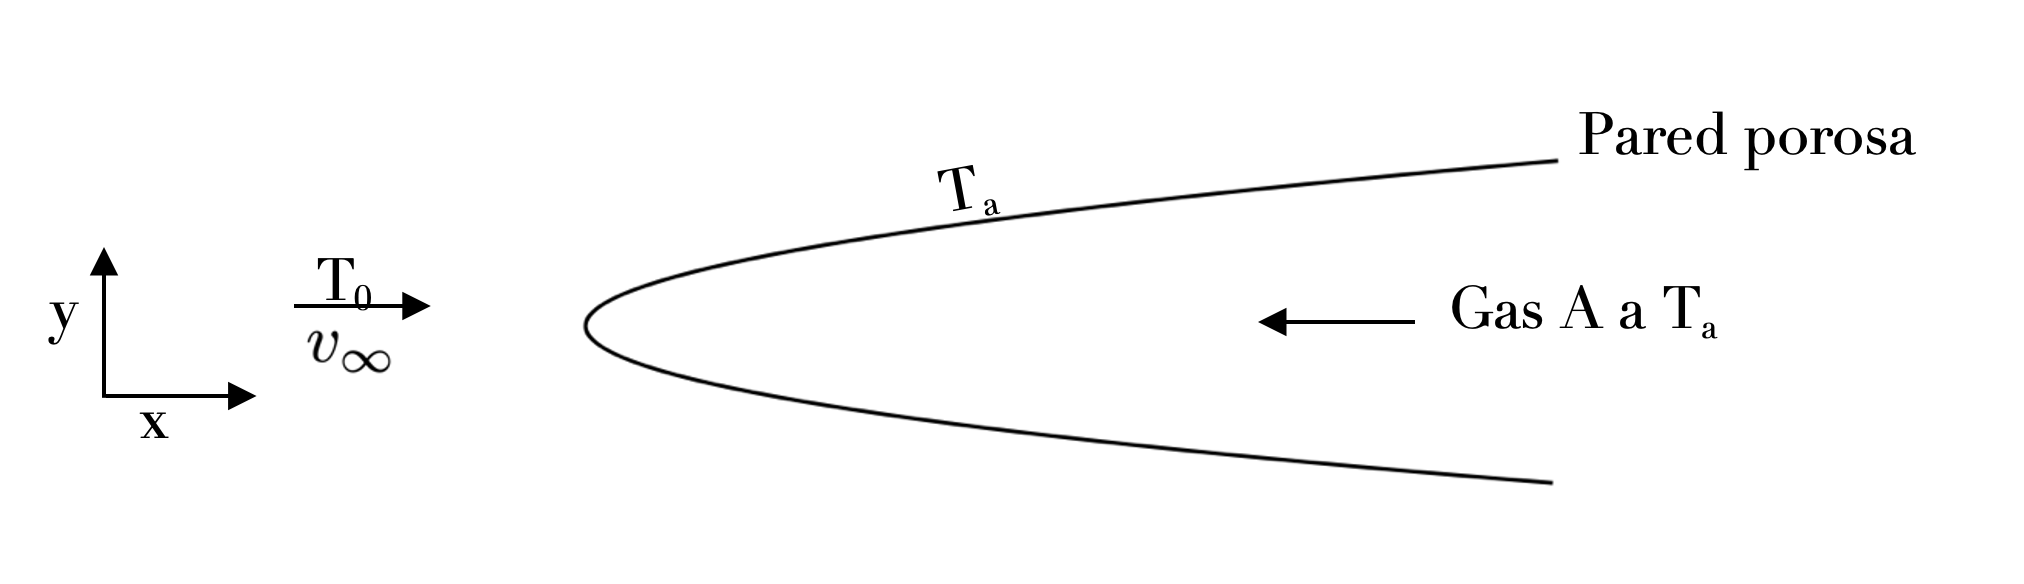
\includegraphics[width=\linewidth]{Capitulo3/Imagenes/Fig_A.1.png}
    \caption{Enfriamiento por transpiración en una placa porosa.}
        \label{fig:Fig_A.1}

\end{figure}

\begin{enumerate}
    \item Evaporación de un líquido A en una corriente de A y B. B es insoluble en A. \newline
    Como $n_{B_0}=0$, $R_w$ en \eqref{eq_A-3} se puede calcular: $R_w=\frac{w_{A_0}-w_{A\infty}}{1-w_{A_0}}$, donde $K=\frac{R_w f''(0)}{Sc}=\frac{1}{Sc}\frac{w_{A_0}-w_{A\infty}}{1-w_{A_0}}f''(0)$
    \item Reacción irreversible de A (gas) en C (sólido) $\to$ B (gas) de acuerdo a $A+C\to 2B$. Pesos moleculares de A y B son iguales. Como $n_{B_0}=-2n_{A_0}$ y $w_A=0$, $R_w=\frac{0-w_{A_\infty}}{-1}=w_{A_\infty}$, donde $K=\frac{1}{Sc}w_{a_\infty f''(0)}$
    \item Enfriamiento por transpiración. Gas A solamente
    \newline 
    Balance de energía:
    \begin{equation*}
        q_0=v_0\hat{C}_p\rho_0(T_a-T_0 )=n_{A_0}\hat{C}_p(T_a-T_0)
    \end{equation*}
    De las ecuaciones \eqref{eq_A-3}: $R_T=\frac{n_{A_0}\hat{C}_p(T_o-T\infty)}{n_{A_0}\hat{C}_p(T_a-T_0)}$
    \newline
    El valor de \( K \) es: \[ K = \frac{1}{Pr} \left( \frac{T_0 - T_\infty}{T_a - T_0} \right) f''(0) \]
\end{enumerate}

\end{document}
